% Preamble
\documentclass[specialist,
    substylefile = spbu_report.rtx,
    subf,href,colorlinks=true, 12pt]{disser}

% Packages
\usepackage[a4paper, includefoot,
    left=3cm, right=1.5cm,
    top=2cm, bottom=2cm,
    headsep=1cm, footskip=1cm]{geometry}
\usepackage{amsmath}
\usepackage{amssymb}
\usepackage[T2A]{fontenc}
\usepackage[utf8]{inputenc}
\usepackage[english, russian]{babel}
\usepackage{pdfpages}
\usepackage{graphicx}
\usepackage{wrapfig}
\usepackage{amsthm}
\usepackage{framed}
\usepackage{xcolor}
\usepackage{color}
\usepackage{fancyvrb}
\usepackage{slashbox}
\usepackage{multirow}
\usepackage{mdwtab}
\usepackage{subcaption}
\usepackage{algorithm}
\usepackage{algorithmicx}
\usepackage{refcount}

%new calligraphic font for subspaces 
\usepackage{euscript}
\newcommand{\cA}{\EuScript{A}}
\newcommand{\cB}{\EuScript{B}}
\newcommand{\cC}{\EuScript{C}}
\newcommand{\cD}{\EuScript{D}}
\newcommand{\cE}{\EuScript{E}}
\newcommand{\cF}{\EuScript{F}}
\newcommand{\cG}{\EuScript{G}}
\newcommand{\cH}{\EuScript{H}}
\newcommand{\cI}{\EuScript{I}}
\newcommand{\cJ}{\EuScript{J}}
\newcommand{\cK}{\EuScript{K}}
\newcommand{\cL}{\EuScript{L}}
\newcommand{\cM}{\EuScript{M}}
\newcommand{\cN}{\EuScript{N}}
\newcommand{\cO}{\EuScript{O}}
\newcommand{\cP}{\EuScript{P}}
\newcommand{\cQ}{\EuScript{Q}}
\newcommand{\cR}{\EuScript{R}}
\newcommand{\cS}{\EuScript{S}}
\newcommand{\cT}{\EuScript{T}}
\newcommand{\cU}{\EuScript{U}}
\newcommand{\cV}{\EuScript{V}}
\newcommand{\cW}{\EuScript{W}}
\newcommand{\cX}{\EuScript{X}}
\newcommand{\cY}{\EuScript{Y}}
\newcommand{\cZ}{\EuScript{Z}}

%font for text indices like transposition X^\mathrm{T}
\newcommand{\rmA}{\mathrm{A}}
\newcommand{\rmB}{\mathrm{B}}
\newcommand{\rmC}{\mathrm{C}}
\newcommand{\rmD}{\mathrm{D}}
\newcommand{\rmE}{\mathrm{E}}
\newcommand{\rmF}{\mathrm{F}}
\newcommand{\rmG}{\mathrm{G}}
\newcommand{\rmH}{\mathrm{H}}
\newcommand{\rmI}{\mathrm{I}}
\newcommand{\rmJ}{\mathrm{J}}
\newcommand{\rmK}{\mathrm{K}}
\newcommand{\rmL}{\mathrm{L}}
\newcommand{\rmM}{\mathrm{M}}
\newcommand{\rmN}{\mathrm{N}}
\newcommand{\rmO}{\mathrm{O}}
\newcommand{\rmP}{\mathrm{P}}
\newcommand{\rmQ}{\mathrm{Q}}
\newcommand{\rmR}{\mathrm{R}}
\newcommand{\rmS}{\mathrm{S}}
\newcommand{\rmT}{\mathrm{T}}
\newcommand{\rmU}{\mathrm{U}}
\newcommand{\rmV}{\mathrm{V}}
\newcommand{\rmW}{\mathrm{W}}
\newcommand{\rmX}{\mathrm{X}}
\newcommand{\rmY}{\mathrm{Y}}
\newcommand{\rmZ}{\mathrm{Z}}

%tt font for time series
\newcommand{\tA}{\mathsf{A}}
\newcommand{\tB}{\mathsf{B}}
\newcommand{\tC}{\mathsf{C}}
\newcommand{\tD}{\mathsf{D}}
\newcommand{\tE}{\mathsf{E}}
\newcommand{\tF}{\mathsf{F}}
\newcommand{\tG}{\mathsf{G}}
\newcommand{\tH}{\mathsf{H}}
\newcommand{\tI}{\mathsf{I}}
\newcommand{\tJ}{\mathsf{J}}
\newcommand{\tK}{\mathsf{K}}
\newcommand{\tL}{\mathsf{L}}
\newcommand{\tM}{\mathsf{M}}
\newcommand{\tN}{\mathsf{N}}
\newcommand{\tO}{\mathsf{O}}
\newcommand{\tP}{\mathsf{P}}
\newcommand{\tQ}{\mathsf{Q}}
\newcommand{\tR}{\mathsf{R}}
\newcommand{\tS}{\mathsf{S}}
\newcommand{\tT}{\mathsf{T}}
\newcommand{\tU}{\mathsf{U}}
\newcommand{\tV}{\mathsf{V}}
\newcommand{\tW}{\mathsf{W}}
\newcommand{\tX}{\mathsf{X}}
\newcommand{\tY}{\mathsf{Y}}
\newcommand{\tZ}{\mathsf{Z}}

%bf font for matrices
\newcommand{\bfA}{\mathbf{A}}
\newcommand{\bfB}{\mathbf{B}}
\newcommand{\bfC}{\mathbf{C}}
\newcommand{\bfD}{\mathbf{D}}
\newcommand{\bfE}{\mathbf{E}}
\newcommand{\bfF}{\mathbf{F}}
\newcommand{\bfG}{\mathbf{G}}
\newcommand{\bfH}{\mathbf{H}}
\newcommand{\bfI}{\mathbf{I}}
\newcommand{\bfJ}{\mathbf{J}}
\newcommand{\bfK}{\mathbf{K}}
\newcommand{\bfL}{\mathbf{L}}
\newcommand{\bfM}{\mathbf{M}}
\newcommand{\bfN}{\mathbf{N}}
\newcommand{\bfO}{\mathbf{O}}
\newcommand{\bfP}{\mathbf{P}}
\newcommand{\bfQ}{\mathbf{Q}}
\newcommand{\bfR}{\mathbf{R}}
\newcommand{\bfS}{\mathbf{S}}
\newcommand{\bfT}{\mathbf{T}}
\newcommand{\bfU}{\mathbf{U}}
\newcommand{\bfV}{\mathbf{V}}
\newcommand{\bfW}{\mathbf{W}}
\newcommand{\bfX}{\mathbf{X}}
\newcommand{\bfY}{\mathbf{Y}}
\newcommand{\bfZ}{\mathbf{Z}}

%bb font for standard spaces and expectation
\newcommand{\bbA}{\mathbb{A}}
\newcommand{\bbB}{\mathbb{B}}
\newcommand{\bbC}{\mathbb{C}}
\newcommand{\bbD}{\mathbb{D}}
\newcommand{\bbE}{\mathbb{E}}
\newcommand{\bbF}{\mathbb{F}}
\newcommand{\bbG}{\mathbb{G}}
\newcommand{\bbH}{\mathbb{H}}
\newcommand{\bbI}{\mathbb{I}}
\newcommand{\bbJ}{\mathbb{J}}
\newcommand{\bbK}{\mathbb{K}}
\newcommand{\bbL}{\mathbb{L}}
\newcommand{\bbM}{\mathbb{M}}
\newcommand{\bbN}{\mathbb{N}}
\newcommand{\bbO}{\mathbb{O}}
\newcommand{\bbP}{\mathbb{P}}
\newcommand{\bbQ}{\mathbb{Q}}
\newcommand{\bbR}{\mathbb{R}}
\newcommand{\bbS}{\mathbb{S}}
\newcommand{\bbT}{\mathbb{T}}
\newcommand{\bbU}{\mathbb{U}}
\newcommand{\bbV}{\mathbb{V}}
\newcommand{\bbW}{\mathbb{W}}
\newcommand{\bbX}{\mathbb{X}}
\newcommand{\bbY}{\mathbb{Y}}
\newcommand{\bbZ}{\mathbb{Z}}

%got font for any case
\newcommand{\gA}{\mathfrak{A}}
\newcommand{\gB}{\mathfrak{B}}
\newcommand{\gC}{\mathfrak{C}}
\newcommand{\gD}{\mathfrak{D}}
\newcommand{\gE}{\mathfrak{E}}
\newcommand{\gF}{\mathfrak{F}}
\newcommand{\gG}{\mathfrak{G}}
\newcommand{\gH}{\mathfrak{H}}
\newcommand{\gI}{\mathfrak{I}}
\newcommand{\gJ}{\mathfrak{J}}
\newcommand{\gK}{\mathfrak{K}}
\newcommand{\gL}{\mathfrak{L}}
\newcommand{\gM}{\mathfrak{M}}
\newcommand{\gN}{\mathfrak{N}}
\newcommand{\gO}{\mathfrak{O}}
\newcommand{\gP}{\mathfrak{P}}
\newcommand{\gQ}{\mathfrak{Q}}
\newcommand{\gR}{\mathfrak{R}}
\newcommand{\gS}{\mathfrak{S}}
\newcommand{\gT}{\mathfrak{T}}
\newcommand{\gU}{\mathfrak{U}}
\newcommand{\gV}{\mathfrak{V}}
\newcommand{\gW}{\mathfrak{W}}
\newcommand{\gX}{\mathfrak{X}}
\newcommand{\gY}{\mathfrak{Y}}
\newcommand{\gZ}{\mathfrak{Z}}

%old calligraphic font
\newcommand{\calA}{\mathcal{A}}
\newcommand{\calB}{\mathcal{B}}
\newcommand{\calC}{\mathcal{C}}
\newcommand{\calD}{\mathcal{D}}
\newcommand{\calE}{\mathcal{E}}
\newcommand{\calF}{\mathcal{F}}
\newcommand{\calG}{\mathcal{G}}
\newcommand{\calH}{\mathcal{H}}
\newcommand{\calI}{\mathcal{I}}
\newcommand{\calJ}{\mathcal{J}}
\newcommand{\calK}{\mathcal{K}}
\newcommand{\calL}{\mathcal{L}}
\newcommand{\calM}{\mathcal{M}}
\newcommand{\calN}{\mathcal{N}}
\newcommand{\calO}{\mathcal{O}}
\newcommand{\calP}{\mathcal{P}}
\newcommand{\calQ}{\mathcal{Q}}
\newcommand{\calR}{\mathcal{R}}
\newcommand{\calS}{\mathcal{S}}
\newcommand{\calT}{\mathcal{T}}
\newcommand{\calU}{\mathcal{U}}
\newcommand{\calV}{\mathcal{V}}
\newcommand{\calW}{\mathcal{W}}
\newcommand{\calX}{\mathcal{X}}
\newcommand{\calY}{\mathcal{Y}}
\newcommand{\calZ}{\mathcal{Z}}


\setcounter{tocdepth}{2}
\graphicspath{{./img}}

\theoremstyle{plain}
\newtheorem{statement}{Утверждение}[section]
\newtheorem{theorem}{Теорема}
\newtheorem{corollary}{Следствие}[statement]

\theoremstyle{definition}
\newtheorem{definition}{Определение}[section]
\newtheorem{property}{Свойство}[section]
\newtheorem{example}{Пример}[section]

\theoremstyle{remark}
\newtheorem*{remark}{Замечание}

\newcommand{\Input}{\textbf{Входные данные: }}
\newcommand{\Output}{\textbf{Результат: }}

\floatname{algorithm}{Алгоритм}
\renewcommand{\listalgorithmname}{Список алгоритмов}

% Document
\begin{document}

    \title{Учебная практика 4 (научно-исследовательская работа) (семестр 7)}
    \topic{<<Тензорный анализ сингулярного спектра>>}
    \author{Хромов Никита Андреевич}
    \date{\number\year}
    \institution{
        Санкт-Петербургский государственный университет\\
        Прикладная математика и информатика
    }
    \group{20.Б04-мм}
    \sa       {Голяндина~Н.\,Э.}
    \sastatus {д.\,ф.-м.\,н., доцент}
    \city{Санкт-Петербург}
    \maketitle

    \tableofcontents


    \section{Введение}\label{sec:intro}
    Singular spectrum analysis (SSA)~\cite{ssa} является популярным методом анализа временных рядов.
    Этот метод используется, в частности, для выделения сигнала и выделения тренда и периодических компонент из временного ряда.
    Метод SSA основан на сингулярном разложении особой матрицы построенной по временному ряду, называемой траекторной.

    В работах~\cite{TSSA, TSSA-improved, hosvd-hooi-separation} предлагается обобщение метода SSA, Tensor SSA, который основан на некотором
    тензорном разложении траекторного тензора, построенного по временному ряду.
    В работах~\cite{TSSA, TSSA-improved} рассматривается задача выделения сигнала из временного ряда,
    а в работе~\cite{hosvd-hooi-separation} "--- задача оценки частот периодических компонент сигнала.
    Причём, в этих работах утверждается о преимуществах Tensor SSA над обычным SSA\@.

    Существует множество видов тензорных разложений, например High-Order Singular Value Decomposition (HOSVD)~\cite{hosvd},
    Canonical Polyadic Decomposition (CPD)~\cite{parafac1, parafac2}, Tucker decomposition~\cite{tucker}.
    В частности, в работах~\cite{TSSA, TSSA-improved} используется разложение CPD, а в
    работе~\cite{hosvd-hooi-separation} "--- HOSVD\@.

    Была поставлена задача изучить различные варианты тензорных разложений, реализовать метод Tensor SSA, выбрав некоторые из них,
    и сравнить с методом Basic SSA по точности выделения сигнала и компонент сигнала, а также
    рассмотреть расширение метода SSA на многомерные ряды "--- метод MSSA~\cite{ssa-2020},
    сформулировать и реализовать тензорную модификацию этого метода и сравнить её с другими методами
    семейства SSA по точности выделения сигнала.
    В качестве первого метода разложения был выбран метод HOSVD, который является обобщением метода SVD для матриц.

    Способ построения траекторного тензора и его разложение были выбраны из предложенных в
    статье~\cite{hosvd-hooi-separation}, однако в отличие от этой статьи, в этой работе изучается применение
    выбранных средств в задаче выделения сигнала из временного ряда и в задаче отделения компонент сигнала.

    В разделе~\ref{sec:hosvd} приведено описание разложения HOSVD и некоторые свойства этого разложения,
    необходимые для доказательства ключевых утверждений о тензорных модификациях SSA.
    В разделах~\ref{sec:HO-SSA-method-description},~\ref{sec:HO-SSA-properties} представлено описание
    тензорных модификаций метода SSA "--- HOSVD SSA и HOOI SSA (оба этих метода в совокупности будем называть
    High-Order SSA или HO-SSA), и приведены утверждения, позволяющие применять некоторые определения и
    свойства из теории базового SSA к модифицированным алгоритмам.
    В разделе~\ref{sec:tensor-ssa-examples} приведены примеры применения методов HO-SSA в задачах выделения сигнала
    из ряда и отделения компонент и численные сравнения этих методов с Basic SSA. По итогам этого раздела была
    выявлена проблема сложности сопоставления компонент разложения с компонентами сигнала, и было установлено,
    что в большинстве рассмотренных случаев методы HO-SSA имеют меньшую точность, чем метод Basic SSA.
    В ходе работы в этом семестре были добавлены
    разделы~\ref{sec:Tensor-MSSA-method-description},~\ref{sec:hosvd-mssa-properties} и~\ref{sec:numerical-compar},
    в которых описывается тензорная модификация метода MSSA "--- HOSVD MSSA и проводятся численные сравнения этого метода
    с известными.
    В результате были получены утверждения, позволяющие применять метод HOSVD MSSA для выделения сигнала, и
    установлено преимущество этого метода над методом MSSA.
    \newpage


    \section{HOSVD и его свойства}\label{sec:hosvd}
    Ключевым этапом в алгоритме HO-SSA является применение тензорного разложения HOSVD~\cite{hosvd} к некоторому тензору.
    Приведём определение этого разложения и некоторые его свойства.
    Все утверждения из этого раздела и их доказательства приведены в статье~\cite{hosvd}.

    \begin{definition}[Произведение тензора и матрицы по измерению]
        Пусть $\mathcal A$ "--- тензор размерности $I_1\times I_2\times\ldots\times I_M$, $\mathbf U$
        "--- матрица размерности $J_n\times I_n$, тогда произведением тензора $\mathcal{A}$ и матрицы $\mathbf{U}$ по
        измерению $n$ $(\mathcal{A}\times_n \mathbf U)$ называется тензор размерности $I_1\times I_2\times\ldots\times I_{n-1}
        \times J_n\times I_{n+1}\times \ldots\times I_M$, который считается по формуле
        \[
            (\mathcal{A}\times_n \mathbf U)_{i_1 i_2\ldots i_{n-1}j_n i_{n+1}\ldots i_M} = \sum_{i_n=1}^{I_n} a_{i_1 i_2\ldots
            i_{n-1}i_n i_{n+1} \ldots i_M} u_{j_n i_n}.
        \]
    \end{definition}

    \begin{theorem}
    [Сингулярное разложение порядка $M$]
        Любой комплекснозначный тензор $\mathcal{A}$ размерности $I_1\times I_2 \times \ldots \times I_M$ может быть представлен
        в виде произведения
        \begin{equation}
            \mathcal{A} = \mathcal{Z} \times_1 \mathbf{U}^{(1)} \times_2 \mathbf{U}^{(2)} \times_3 \ldots \times_M \mathbf{U}^{(M)},\label{eq:hosvd}
        \end{equation}
        в котором
        \begin{enumerate}
            \item $\mathbf{U}^{(n)}=\left[U_1^{(n)}:\, U_2^{(n)}:\ldots:\, U_{I_n}^{(n)} \right]$ "--- унитарная матрица,
            \item $\mathcal{Z}$ "--- комплекснозначный тензор размерности $I_1\times I_2 \times \ldots \times I_M$, в котором
            каждый подтензор $\mathcal Z_{i_n=\alpha}$, полученный фиксированием индекса $i_n=\alpha$ удовлетворяет следующим свойствам
            \begin{enumerate}
                \item полная ортогональность: подтензоры $\mathcal Z_{i_n=\alpha}$ и $\mathcal Z_{i_n=\beta}$ ортогональны для всех возможных значений
                $n,\, \alpha,\, \beta: \alpha\ne\beta$:
                \[
                    \langle\mathcal Z_{i_n=\alpha},\mathcal Z_{i_n=\beta}\rangle=0 \qquad \alpha\ne\beta,
                \]
                \item упорядоченность: подтензоры расположены в порядке убывания их норм Фробениуса:
                \begin{equation}
                    \|\mathcal Z_{i_n=1}\|\geqslant\|\mathcal Z_{i_n=2}\| \geqslant \ldots \geqslant\|\mathcal Z_{i_n=I_n}\|\label{eq:order}
                \end{equation}
                для всех $n\in \overline{1:M}$.
            \end{enumerate}
        \end{enumerate}
    \end{theorem}
    \begin{definition}[Сингулярное разложение тензора]
        \label{def:hosvd}
        Разложение вида~\eqref{eq:hosvd} будем называть сингулярным разложением тензора $\mathcal{A}$ порядка $M$ или
        HOSVD тензора $\mathcal{A}$.
    \end{definition}
    \begin{definition}[Сингулярное число тензора]
        \label{def:singular-value}
        Обозначим $\sigma_i^{(n)}=\|\mathcal Z_{i_n=i}\|$ и будем называть $\sigma_i^{(n)}$ $i$-м сингулярным числом
        тензора $\mathcal A$ по измерению $n$.
    \end{definition}
    \begin{definition}[Сингулярный вектор тензора]
        \label{def:singular-tensor}
        Векторы $U_i^{(n)}$ будем называть $i$-м сингулярным вектором тензора $\mathcal A$ по измерению $n$.
    \end{definition}
    \begin{remark}
        Представление~\eqref{eq:hosvd} можно записать в виде
        \begin{equation}
            \mathcal{A}=\sum_{i_1=1}^{I_1} \sum_{i_2=1}^{I_2}\ldots \sum_{i_M=1}^{I_M} \mathcal{Z}_{i_1,i_2,\ldots,i_M}
            U^{(1)}_{i_1} \circ U^{(2)}_{i_2} \circ \ldots\circ U^{(M)}_{i_M}.\label{eq:sum-hosvd}
        \end{equation}
        Такое представление удобнее для описания алгоритма HO-SSA\@.
    \end{remark}

    \subsection{Свойства HOSVD}\label{subsec:hosvd-properties}
    Многие свойства метода SSA являются следствиями свойств SVD\@.
    В свою очередь, многие свойства HOSVD являются аналогами свойств SVD\@.
    Таким образом, аналогичность свойств SSA и HO-SSA может быть выведена из аналогичности некоторых свойств SVD и HOSVD\@.
    \begin{definition}[Развёртка тензора по измерению]
        Пусть $\mathcal{A}$ "--- тензор размерности $I_1\times I_2\times\ldots\times I_M$, тогда его развёртка
        по $n$-му измерению "--- это матрица $\mathbf{A}_{(n)}$ (или $[\bfA]_n$)
        размерности $I_n\times I_{n+1}I_{n+2}\ldots I_{M}I_{1}I_{2}\ldots I_{n-1}$,
        в которой элемент $a_{i_1 i_2\ldots i_M}$ тензора содержится в строке $i_n$ и столбце с номером равным
        \[\begin{aligned}
              &(i_{n+1} - 1)I_{n+2}I_{n+3}\ldots I_{M}I_1 I_2\ldots I_{n-1} + (i_{n+2} - 1)I_{n+3}I_{n+4}\ldots I_M I_1 I_2 \ldots
              I_{n-1} + \dots \\
              &+(i_M - 1)I_1 I_2 \ldots I_{n-1} + (i_1 - 1)I_2 I_3\ldots I_{n-1} + (i_2 - 1)I_3 I_4\ldots I_{n-1} + \dots + i_{n-1}.
        \end{aligned}
        \]

        \begin{figure}[!h]
            \centering
            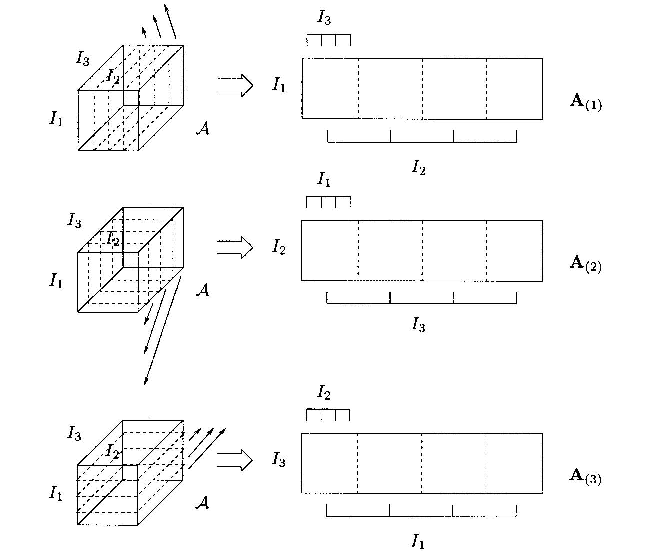
\includegraphics[width=\textwidth]{unfolding}
            \caption{Развёртка тензора $\mathcal{A}$ размерности $I_1\times I_2 \times I_3$ в матрицы $\mathbf{A}_{(1)},\,
            \mathbf{A}_{(2)},\, \mathbf{A}_{(3)}$ размерностей $I_1\times (I_2 I_3),\, I_2\times (I_3 I_1),\, I_3\times (I_1 I_2)$
                соответственно}
            \label{fig:unfolding}
        \end{figure}
    \end{definition}

    Пусть $\calA$ "--- тензор размерности $I_1\times I_2\times\ldots\times I_M$, применим SVD к развёрткам этого тензора вдоль каждого
    измерения, в результате чего получим $M$ матриц $\mathbf{U}^{(n)}$,
    составленных из левых сингулярных векторов соответствующих развёрток.
    Теперь определим тензор $\calZ$ следующим образом
    \[
        \mathcal{Z}=\mathcal{A}\times_1 \mathbf{U}^{(1)^\mathrm{H}}\times_2 \mathbf{U}^{(2)^\mathrm{H}}\ldots \times_M
        \mathbf{U}^{(M)^\mathrm{H}}.
    \]
    Тогда исходный тензор $\calA$ можно представить в виде
    \begin{equation}
        \label{eq:hosvd-to-svd}
        \mathcal{A} = \mathcal{Z}\times_1 \mathbf{U}^{(1)}\times_2 \mathbf{U}^{(2)}\ldots \times_M \mathbf{U}^{(M)}.
    \end{equation}

    \begin{statement}
        Представление тензора $\calA$ в виде~\eqref{eq:hosvd-to-svd} является HOSVD этого тензора.
        \label{state:hosvd-to-svd}
    \end{statement}

    Из-за этой связи HOSVD со стандартным матричным SVD для многих свойств SVD существуют аналогичные свойства HOSVD\@.
    \begin{property}[Единственность]
        \leavevmode
        \begin{enumerate}
            \item Все сингулярные числа по каждому измерению определяются однозначно.
            \item Если сингулярные числа по измерению $n$ различны, то сингулярные векторы по измерению $n$ определены
            в точности до умножения на коэффициент единичной нормы.
            Если $U_\alpha^{(n)}$ умножается на $e^{i\theta}$, то $\mathcal{Z}_{i_n=\alpha}$ должен быть умножен на обратный
            коэффициент $e^{-i\theta}$.
        \end{enumerate}
        Сингулярные векторы по измерению $n$, соответствующие одному и тому же сингулярному числу по измерению $n$,
        могут быть заменены любой унитарной линейной комбинацией.
        Соответствующие подтензоры $\{\mathcal{Z}_{i_n=\alpha}\}$ должны быть пересчитаны обратным образом.
        Формально $\mathbf{U}^{(n)}$ можно заменить на $\mathbf{U}^{(n)}\mathbf{Q}$, где $\mathbf{Q}$ "--- блочно-диагональная
        матрица, состоящая из унитарных блоков, в которой блочное разбиение соответствует разбиению $\mathbf{U}^{(n)}$
        на наборы сингулярных векторов по измерению $n$, соответствующих одинаковым сингулярным значениям по измерению $n$.
        При этом тензор $\mathcal{Z}$ должен быть заменён на $\mathcal{Z}\times_{n} \mathbf{Q}^{\mathrm{H}}$.

        В случае вещественнозначных тензоров единственность имеется в точности до знака, что соответствует
        умножению на унитарную матрицу.
    \end{property}

    \begin{property}[Обобщение]
        HOSVD тензора второго порядка сводится к его матричному SVD\@.
    \end{property}
    Это свойство означает, что результат применения HOSVD к тензору с двумя измерениями, т.е. матрице, совпадает
    с результатом применения SVD к этой же матрице, в точности до унитарных преобразований сингулярных векторов и
    матрицы сингулярных значений.

    Перед формулировкой следующих свойств необходимо ввести несколько определений.
    \begin{definition}[$n$-ранг]
        $n$-рангом тензора $\mathcal{A}$ называется размерность векторного пространства, порождённого векторами измерения $n$ этого тензора.
        Обозначается $R_n=\operatorname{rank}_{n}(\mathcal{A})$.
    \end{definition}

    \begin{remark}
        В отличие от матричного случая, $n$-ранги тензора порядка выше $2$ могут в общем случае отличаться.
    \end{remark}

    \begin{definition}[Тензорный ранг]
        \leavevmode
        \begin{enumerate}
            \item Говорят, что тензор $\mathcal{A}$ размерности $I_1\times I_2\times \ldots \times I_M$ имеет тензорный ранг равный $1$, если он представим в виде
            \[
                \mathcal{A}=a_1\circ a_2\circ \ldots \circ a_M,
            \]
            где $a_{k} \in \mathbb{C}^{I_k}$, а $\circ$ обозначает внешнее произведение.
            \item Говорят, что тензор $\mathcal{A}$ имеет ранг $R$, если он представим в виде линейной комбинации $R$ тензоров
            ранга $1$, и такое $R$ минимальное.
            Обозначение: $R=\operatorname{rank}(\mathcal{A})$.
        \end{enumerate}
    \end{definition}

    \begin{remark}
        В общем случае ранг тензора $\mathcal{A}$ не равен его $n$-рангам, даже если они все равны между собой.
        Более того, всегда справедливо неравенство $\operatorname{rank}_n(\mathcal{A})\leqslant \operatorname{rank}(\mathcal{A})$.
    \end{remark}

    \begin{property}
    [Связь $n$-ранга тензора и ранга его развёртки по измерению $n$]
        Векторы измерения $n$ тензора $\mathcal{A}$ являются столбцами его развёртки по измерению $n$ и выполняется равенство
        \[\operatorname{rank}_{n}(\mathcal{A})=\operatorname{rank}(\mathbf{A}_{(n)}).\]
    \end{property}

    \begin{property}
    [Связь $n$-ранга тензора и его HOSVD]
        \label{property:n-rank}
        Пусть имеется HOSVD тензора $\mathcal{A}$ размерности $I_1\times I_2\times \ldots \times I_M$
        \[\mathcal{A} = \mathcal{Z}\times_1 \mathbf{U}^{(1)}\times_2\mathbf{U}^{(2)}\times_3\ldots \times_{M}\mathbf{U}^{(M)},\]
        тогда, по определению, тензор $\mathcal{Z}$ удовлетворяет свойству упорядоченности сингулярных чисел
        \[\|\mathcal{Z}_{i_n=1}\|\geqslant\|\mathcal{Z}_{i_n=2}\|\geqslant\ldots \geqslant \|\mathcal{Z}_{i_n=I_n}\|\]
        для всех $n\in \overline{1:M}$.
        Обозначим $r_n$ "--- наибольший индекс такой, что $\|\mathcal{Z}_{i_n=r_n}\|>0$.
        Тогда
        \begin{equation}
            \operatorname{rank}_n(\mathcal{A})=r_n.\label{eq:n-rank}
        \end{equation}
    \end{property}

    \begin{property}[Норма]
        \label{property:norm}
        Пусть имеется HOSVD тензора $\mathcal{A}$, представленное в виде~\eqref{eq:hosvd}, и пусть $R_n=\operatorname{rank}_n(\mathcal{A})$,
        $n\in \overline{1:M}$.
        Тогда справедливо равенство
        \begin{align*}
            \|\mathcal{A}\|^2&=\sum_{i=1}^{R_1}\left( \sigma_i^{(1)} \right)^2=\sum_{i=1}^{R_2}\left( \sigma_i^{(2)} \right)^2
            =\ldots =\sum_{i=1}^{R_M}\left( \sigma_i^{(M)} \right)^2=\\
            &= \|\mathcal{Z}\|^2.
        \end{align*}
    \end{property}

    \begin{definition}[Ориентированная энергия]
        Ориентированной по измерению $n$ энергией тензора $\mathcal{A}\in \mathbb{C}^{I_1\times I_2\times \ldots \times I_M}$ в направлении
        вектора $X\in \mathbb{C}^{I_n}$ единичной нормы называют выражение
        \[
            \operatorname{OE}_n(X, \mathcal{A}) = \|X^{\mathrm{H}}\mathbf{A}_{(n)}\|^2.
        \]
    \end{definition}

    \begin{property}[Об ориентированной энергии]
        \label{property:oriented-energy}
        Направления экстремальной ориентированной энергии по измерению $n$ соответствуют сингулярным векторам по измерению $n$,
        причем значение экстремальной энергии равно соответствующему квадрату сингулярного значения по измерению $n$.
    \end{property}

    Это означает, что векторы тензора $\mathcal{A}$ по измерению $n$ в основном содержат вклады в направлении $U^{(n)}_1$;
    на это направление приходится $\sigma^{(n)^2}_1$ энергии по отношению к общему количеству энергии в тензоре.
    Затем ориентированная энергия по измерению $n$ достигает экстремума в направлении $U^{(n)}_2$,
    перпендикулярном $U^{(n)}_1$, с величиной $\sigma^{(n)^2}_2$, и так далее.

    \begin{property}[Приближение]
        \label{property:approx}
        Пусть имеется HOSVD тензора $\mathcal{A}$, представленное в виде~\eqref{eq:hosvd}, и пусть $R_n=\operatorname{rank}_n(\mathcal{A})$.
        Определим тензор $\hat{\mathcal{A}}$ отбрасыванием наименьших сингулярных значений $\sigma_{I_{n}'+1}^{(n)}, \sigma_{I_{n}'+2}^{(n)},\ldots, \sigma_{R_n}^{(n)}$
        для заданных значений $I_{n}'$, $n \in \overline{1:M}$, то есть заменяя нулями соответствующие части тензора $\mathcal{Z}$.
        Тогда верно
        \begin{equation}
            \|\mathcal{A}-\hat{\mathcal{A}}\|^2\leqslant \sum_{i_1=I_{1}'+1}^{R_1}\left( \sigma_{i_1}^{(1)}\right)^2 +
            \sum_{i_2=I_{2}'+1}^{R_2}\left( \sigma_{i_2}^{(2)}\right)^2 + \ldots + \sum_{i_M=I_{M}'+1}^{R_M}\left( \sigma_{i_M}^{(M)}\right)^2.\label{eq:approx}
        \end{equation}
    \end{property}

    Это свойство является эквивалентом высшего порядка связи между SVD матрицы и ее наилучшим приближением,
    в смысле наименьших квадратов, матрицей более низкого ранга.
    Однако для тензоров ситуация совершенно иная.
    Отбрасывая наименьшие сингулярные значения измерения $n$, мы получаем тензор $\hat{\mathcal{A}}$ с рангом столбцов
    равным $I_1'$, рангом строк равным $I_2'$ и т.д.
    Но этот тензор в общем случае не является наилучшим приближением при заданных ограничениях на ранги измерений.
    Тем не менее, предположение об упорядочении~\eqref{eq:order} подразумевает, что <<энергия>> $\mathcal{A}$ в основном сосредоточена в части,
    соответствующей малым значениям $i_1, i_2, \ldots, i_M$.
    Следовательно, если $\sigma^{(n)}_{I_n'} \gg \sigma^{(n)}_{I_n'+1}$ (например, если $I_n'=\operatorname{rank}_n(\mathcal{A})$,
    то меньшие сингулярные значения по измерению $n$ не существенны), то $\hat{\mathcal{A}}$ всё ещё можно считать хорошим приближением $\mathcal{A}$.
    Ошибка ограничена выражением~\eqref{eq:approx}.


    \section{Описание метода HO-SSA}\label{sec:HO-SSA-method-description}
    Пусть дан временной ряд $\tX$ длины $N$
    \[
        \tX=(x_1,x_2,\ldots,x_N).
    \]
    \begin{definition}[Траекторный тензор ряда]
        Траекторным тензором ряда $\tX$ с параметрами $I,L: 1\leqslant I,L \leqslant N,\, I + L \leqslant N + 1$
        будем называть тензор $\mathcal{X}$ размерности $I\times L \times J,\, J=N-I-L+2$, элементы которого удовлетворяют равенству
        \[
            \mathcal{X}_{i,l,j}=x_{i+l+j-2}\qquad i\in \overline{1:I},\, l \in\overline{1:L},\, j \in\overline{1:J}.
        \]
    \end{definition}
    \begin{definition}[Оператор вложения]
        \label{def:injection-op}
        Оператором вложения $\calH_L$ с длиной окна $L$ будем называть отображение, переводящее временной ряд
        $\tX=(x_1, x_2,\ldots, x_N)$, $N \geqslant L$, в матрицу $\bfX$ размерности $L\times K$, $K = N-L+1$,
        такую, что $\bfX_{l,k}=x_{l+k-1}$.

        Другими словами
        \[
            \calH_L(\tX) =
            \begin{pmatrix}
                x_1    & x_2     & \ldots & x_K     \\
                x_2    & x_3     & \ldots & x_{K+1} \\
                \vdots & \vdots  & \ddots & \vdots  \\
                x_L    & x_{L+1} & \ldots & x_N
            \end{pmatrix}.
        \]
    \end{definition}

    В терминах оператора вложения слои траекторного тензора ряда $\tX$
    с параметрами $I, L$ имеют следующий вид
    \begin{gather*}
        \mathcal{X}_{,,j}= \calH_I \Big((x_j, x_{j+1}, \ldots, x_{j+I+L-2})\Big),\\
        \mathcal{X}_{,l,}= \calH_I \Big((x_l, x_{l+1}, \ldots, x_{l+L+J-2})\Big),\\
        \mathcal{X}_{i,,}=\calH_L \Big((x_i, x_{i+1}, \ldots, x_{i+L+J-2})\Big).\\
    \end{gather*}

    На вход алгоритму подаётся временной ряд $\tX$ и параметры $I,L: 1\leqslant I,L \leqslant N,\, I + L \leqslant N + 1$.
    Так как при замене одного из этих параметров на $J=N-I-L+2$ или при замене их между собой получаются
    те же самые траекторные тензоры с точностью до перестановки их измерений, то имеет смысл при
    рассмотрении нескольких наборов параметров рассматривать только те, которые дают уникальные тройки $(I, L, J)$.
    В зависимости от целей определяются разные формулировки алгоритма.

    HOSVD-SSA для отделения различных компонент ряда друг от друга представлен в алгоритме~\ref{alg:hosvd-ssa-components}
    \begin{algorithm}
        \caption{HOSVD-SSA для отделения компонент ряда.}
        \label{alg:hosvd-ssa-components}
        \Input $\tX$, $I,L: 1\leqslant I,L \leqslant N,\, I + L \leqslant N + 1$, где $N$ "--- длина $\tX$, $m$,
        $\mathfrak{S}_1, \ldots, \mathfrak{S}_m:$
        \[
            \mathfrak{S}=\bigcup_{k=1}^{m}\mathfrak{S}_k \qquad \mathfrak{S}_k\cap \mathfrak{S}_l =\emptyset,\, k\ne l,
        \] где $\mathfrak{S}=\{1,\, 2\,\ldots,\, \min(I, L, J)\}$.\\
        \Output $\tX^{(1)}, \tX^{(2)}, \ldots, \tX^{(m)}$:
        \[
            \tX=\sum_{k=1}^{m}\tX^{(k)}.
        \]
        \begin{algorithmic}[1]
            \State \label{alg:first-step}
            Построение траекторного тензора $\mathcal{X}$ по параметрам $I, L$.
            \State \label{alg:second-step}
            Проведение HOSVD траекторного тензора $\mathcal{X}$, получение его представления в виде~\eqref{eq:sum-hosvd}
            \begin{equation}
                \mathcal{X}=\sum_{i=1}^{I} \sum_{l=1}^{L} \sum_{j=1}^{J} \mathcal{Z}_{i,l,j} \mathbf{U}^{(1)}_{i}
                \circ \mathbf{U}^{(2)}_{l} \circ \mathbf{U}^{(3)}_{j}.
                \label{eq:trajectory-hosvd}
            \end{equation}
            \State Группировка: построение тензоров
            \begin{equation*}
                \mathcal{X}^{(\mathfrak{S}_k)}=\sum_{i \in \mathfrak{S}_k} \sum_{l\in \mathfrak{S}_k} \sum_{j\in \mathfrak{S}_k}
                \mathcal{Z}_{i,l,j} \mathbf{U}^{(1)}_{i}\circ \mathbf{U}^{(2)}_{l} \circ \mathbf{U}^{(3)}_{j}.
%            \label{eq:tens-group}
            \end{equation*}
            \State Восстановление рядов $\tX^{(k)}=\tX^{(\mathfrak{S}_k)}$ по тензорам $\mathcal{X}^{(\mathfrak{S}_k)}$ посредством их усреднения вдоль
            плоскостей $i+l+j=\operatorname{const}$:
            \begin{gather*}
                x^{(k)}_n=\frac{1}{\#\mathfrak{M}_n}\sum_{(i,l,j)\in \mathfrak{M}_n} \mathcal{X}^{(\mathfrak{S}_k)}_{i,l,j},\qquad n\in \overline{1:N},\\
                \mathfrak{M}_n=\{(i,\, l,\, j) | 1\leqslant i \leqslant I,\, 1\leqslant l \leqslant L,\, 1\leqslant j \leqslant J,\, i+l+j-2=n\}.
            \end{gather*}
        \end{algorithmic}
    \end{algorithm}
%    \begin{enumerate}
%        \item Выбор параметров $I, L$ и построение по ним траекторного тензора $\mathcal{X}$;
%        \item Проведение HOSVD траекторного тензора $\mathcal{X}$, получение его представления в виде~\eqref{eq:sum-hosvd}
%        \begin{equation}
%            \mathcal{X}=\sum_{i=1}^{I} \sum_{l=1}^{L} \sum_{j=1}^{J} \mathcal{Z}_{i,l,j} \mathbf{U}^{(1)}_{i}
%            \circ \mathbf{U}^{(2)}_{l} \circ \mathbf{U}^{(3)}_{j};
%            \label{eq:trajectory-hosvd}
%        \end{equation}
%        \item Группировка: разбиение множества индексов $\mathfrak{S}=\{1,\, 2\,\ldots,\, \min(I, L, J)\}$ по смыслу на
%        непересекающиеся множества
%        \[
%            \mathfrak{S}=\bigcup_{k=1}^{m}\mathfrak{S}_k \qquad \mathfrak{S}_k\cap \mathfrak{S}_l =\emptyset,\, k\ne l,
%        \]
%        и построение тензоров
%        \begin{equation*}
%            \mathcal{X}^{(\mathfrak{S}_k)}=\sum_{i \in \mathfrak{S}_k} \sum_{l\in \mathfrak{S}_k} \sum_{j\in \mathfrak{S}_k}
%            \mathcal{Z}_{i,l,j} \mathbf{U}^{(1)}_{i}\circ \mathbf{U}^{(2)}_{l} \circ \mathbf{U}^{(3)}_{j}.
%%            \label{eq:tens-group}
%        \end{equation*}
%        \item Восстановление рядов $\tX^{(k)}=\tX^{(\mathfrak{S}_k)}$ по тензорам $\mathcal{X}^{(\mathfrak{S}_k)}$ посредством их усреднения вдоль
%        плоскостей $i+l+j=\operatorname{const}$:
%        \begin{gather*}
%            x^{(k)}_n=\frac{1}{\#\mathfrak{M}_n}\sum_{(i,l,j)\in \mathfrak{M}_n} \mathcal{X}^{(\mathfrak{S}_k)}_{i,l,j},\qquad n\in \overline{1:N},\\
%            \mathfrak{M}_n=\{(i,\, l,\, j) | 1\leqslant i \leqslant I,\, 1\leqslant l \leqslant L,\, 1\leqslant j \leqslant J,\, i+l+j-2=n\}.
%        \end{gather*}
%    \end{enumerate}
%    Результатом алгоритма является набор временных рядов $\tX^{(1)},\ldots,\, \tX^{(m)}$ такой, что
%    \[
%        \tX=\sum_{k=1}^{m}\tX^{(k)}.
%    \]

    Алгоритм HO-SSA для выделения в ряде сигнала из шума сводится к получению
    как можно более точного приближения траекторного тензора тензором меньшего, заданного пользователем, ранга, и
    может быть проведён двумя различными способами.

    Первый способ заключается в приближении траекторного тензора путём усечения его HOSVD (HOSVD SSA).
    Благодаря свойствам~\ref{property:approx},~\ref{property:oriented-energy} такое приближение можно считать достаточно точным,
    хоть оно и не оптимально.
    Первые два шага этого алгоритма совпадают с алгоритмом для отделения компонент ряда, поэтому опишем его, начиная с третьего шага.
    Описание приведено в алгоритме~\ref{alg:hosvd-ssa-signal}.

    \begin{algorithm}
        \caption{HOSVD SSA для выделения сигнала.}
        \label{alg:hosvd-ssa-signal}
        \Input $\tX$, $I,L: 1\leqslant I,L \leqslant N,\, I + L \leqslant N + 1$, где $N$ "--- длина $\tX$, $R_1 \in \overline{1:I}$,
        $R_2 \in \overline{1:L}$, $R_3 \in \overline{1:J}$.\\
        \Output $\hat{\tX}$.

        \begin{algorithmic}[1]
            \setcounterref{ALG@line}{alg:second-step}
            \State По параметрам $R_1, R_2, R_3$ и разложению траекторного тензора $\mathcal{X}$
            в виде~\eqref{eq:trajectory-hosvd},
            в тензоре $\mathcal{Z}$ проводится замена матриц-слоёв с номерами $k>R_m$ в соответствующих измерениях
            на нулевые, и по полученному тензору $\hat{\mathcal{Z}}$
            строится приближение траекторного тензора $\hat{\mathcal{X}}$.
            \State Усреднение тензора $\hat{\mathcal{X}}$ вдоль плоскостей $i+l+j=\operatorname{const}$,
            в результате чего получается оценка сигнала $\hat{\tX}$.
        \end{algorithmic}
    \end{algorithm}
%    \begin{enumerate}
%        \setcounter{enumi}{2}
%        \item Третий шаг заключается в выборе ранга сигнала $r$ и усечении тензора сингулярных значений по этому рангу.
%        Другими словами, имея ранг сигнала $r$ и разложение траекторного тензора $\mathcal{X}$ в виде~\eqref{eq:trajectory-hosvd},
%        в тензоре $\mathcal{Z}$ заменим матрицы-слои по каждому измерению с номерами $k>r$ на нулевые, и по полученному тензору $\hat{\mathcal{Z}}$
%        построим приближение траекторного тензора $\hat{\mathcal{X}}$.
%        \item На четвёртом шаге, используя усреднение тензора $\hat{\mathcal{X}}$ вдоль плоскостей $i+l+j=\operatorname{const}$
%        получим ряд $\hat{\tX}$.
%        Этот ряд и будем считать сигналом.
%    \end{enumerate}

    Второй способ использует метод приближения тензора другим тензором с меньшими значениями $n$-рангов "--- High-Order Orthogonal
    Iteration (HOOI)~\cite{hooi}.
    При заданных тензоре $\mathcal{A}$ и наборе $n$-рангов $(R_1,\, R_2,\, \ldots,\, R_M)$, результатом метода будет
    тензор $\hat{\mathcal{A}}$, $n$-ранги которого совпадают с набором $(R_1,\, R_2,\, \ldots,\, R_M)$, и который решает
    задачу минимизации
    \[
        \|\mathcal{A}-\hat{\mathcal{A}}\|\to \min,
    \]
    где минимум берётся по классу тензоров с заданными $n$-рангами.
    Исходя из определения, результат метода HOOI является оптимальным, в связи с чем его можно использовать
    для приближения траекторного тензора ряда.

    Приведём вторую реализацию алгоритма HO-SSA для отделения сигнала от шума, используя HOOI (HOOI SSA).
    Первый шаг алгоритма совпадает с предыдущими алгоритмами, поэтому опишем его начиная со второго шага.
    Описание приведено в алгоритме~\ref{alg:hooi-ssa}.

    \begin{algorithm}
        \caption{HOOI SSA}
        \label{alg:hooi-ssa}
        \Input $\tX$, $I,L: 1\leqslant I,L \leqslant N,\, I + L \leqslant N + 1$, где $N$ "--- длина $\tX$, $R_1 \in \overline{1:I}$,
        $R_2 \in \overline{1:L}$, $R_3 \in \overline{1:J}$.\\
        \Output $\hat{\tX}$.

        \begin{algorithmic}[1]
            \setcounterref{ALG@line}{alg:first-step}
            \State Применение к построенному на первом шаге траекторному тензору $\mathcal{X}$ алгоритма
            HOOI с набором $n$-рангов $(R_1,\, R_2,\, R_3)$, в результате чего получается тензор $\hat{\calX}$.
            \State Восстановление сигнала по тензору $\hat{\mathcal{X}}$ совпадает с четвёртым шагом в
            алгоритме HOSVD SSA для выделения в ряде сигнала из шума.
        \end{algorithmic}
    \end{algorithm}
%    \begin{enumerate}
%        \setcounter{enumi}{1}
%        \item На втором шаге выбирается ранг сигнала $r$ и к полученному ранее траекторному тензору $\mathcal{X}$ применяется
%        HOOI с набором $n$-рангов $(r,\, r,\, r)$.
%        В результате получаем оптимальное приближение траекторного тензора $\mathcal{X}$ тензором $\hat{\mathcal{X}}$ со
%        значениями $n$-рангов равными $r$.
%        \item Третий шаг "--- восстановление ряда по тензору $\hat{\mathcal{X}}$ совпадает с четвёртым шагом в
%        алгоритме HOSVD SSA для выделения в ряде сигнала из шума.
%    \end{enumerate}


    \section{Свойства HO-SSA}\label{sec:HO-SSA-properties}
    В силу аналогичности свойств SVD и HOSVD, многие определения и свойства из теории SSA~\cite{ssa} можно перенести на тензорный случай.

    \subsection{Разделимость рядов в терминах HO-SSA}\label{subsec:tensor-ssa-separability}
    \begin{statement}
        \label{state:separability}
        $\tilde{\tX}=(\tilde{x}_1,\ldots , \tilde{x}_N)$, $\hat{\tX}=(\hat{x}_1,\ldots , \hat{x}_N)$ "--- временные ряды длины $N$.
        Пусть ряд $\tX$ является суммой этих рядов.
        Траекторные тензоры рядов равны соответственно: $\tilde{\mathcal{X}},\, \hat{\mathcal{X}},\, \mathcal{X}$.
        Тогда существует сингулярное разложение тензора $\mathcal{X}$ с параметрами $I, L$, которое можно представить
        в виде суммы сингулярных разложений тензоров $\tilde{\mathcal{X}}$ и $\hat{\mathcal{X}}$ с теми же параметрами
        в том и только том случае, когда взаимно ортогональны все подряды рядов $\tilde{\tX}$ и $\hat{\tX}$
        длины $I,\, L,\, J=N-I-L+2$, то есть
        \begin{enumerate}
            \item $\tilde{x}_{k}\hat{x}_m + \ldots + \tilde{x}_{k+I-1} \hat{x}_{m+I-1}=0 \qquad \forall k,\, m\in\overline{1:N-I+1}$,
            \item $\tilde{x}_{k}\hat{x}_m + \ldots + \tilde{x}_{k+L-1} \hat{x}_{m+L-1}=0 \qquad \forall k,\, m\in\overline{1:N-L+1}$,
            \item $\tilde{x}_{k}\hat{x}_m + \ldots + \tilde{x}_{k+J-1} \hat{x}_{m+J-1}=0 \qquad \forall k,\, m\in\overline{1:N-J+1}$.
        \end{enumerate}
    \end{statement}
    \begin{proof}
        Сингулярные разложения тензоров $\mathcal{X}, \tilde{\mathcal{X}}, \hat{\mathcal{X}}$ могут быть представлены в виде
        следующих сумм:
        \[
            \begin{aligned}
                \mathcal{X}=\sum_{i=1}^{I} \sum_{l=1}^{L} \sum_{j=1}^{J} \mathcal{Z}_{i,l,j} \mathbf{U}^{(1)}_{i}
                \circ \mathbf{U}^{(2)}_{l} \circ \mathbf{U}^{(3)}_{j},\\
                \tilde{\mathcal{X}}=\sum_{i=1}^{I} \sum_{l=1}^{L} \sum_{j=1}^{J} \tilde{\mathcal{Z}}_{i,l,j}
                \tilde{\mathbf{U}}^{(1)}_{i} \circ \tilde{\mathbf{U}}^{(2)}_{l} \circ \tilde{\mathbf{U}}^{(3)}_{j},\\
                \hat{\mathcal{X}}=\sum_{i=1}^{I} \sum_{l=1}^{L} \sum_{j=1}^{J} \hat{\mathcal{Z}}_{i,l,j}
                \hat{\mathbf{U}}^{(1)}_{i} \circ \hat{\mathbf{U}}^{(2)}_{l} \circ \hat{\mathbf{U}}^{(3)}_{j}.
            \end{aligned}
        \]

        Сумма $\mathcal{X} = \sum_{i} \sum_{l} \sum_{j} \tilde{\mathcal{Z}}_{i,l,j}
        \tilde{\mathbf{U}}^{(1)}_{i} \circ \tilde{\mathbf{U}}^{(2)}_{l} \circ \tilde{\mathbf{U}}^{(3)}_{j} +
        \sum_{i} \sum_{l} \sum_{j} \hat{\mathcal{Z}}_{i,l,j} \hat{\mathbf{U}}^{(1)}_{i} \circ \hat{\mathbf{U}}^{(2)}_{l}
        \circ \hat{\mathbf{U}}^{(3)}_{j}$ является сингулярным разложением $\mathcal{X}$ в том и только том случае, когда
        пары векторов $\tilde{\mathbf{U}}^{(\sigma)}_{k},\, \hat{\mathbf{U}}^{(\sigma)}_{m}$ взаимно ортогональны
        при всех возможных значениях $\sigma, k, m$.
        Это равносильно ортогональности линейных пространств $\mathcal{L}^{(\sigma)}_{1},\, \mathcal{L}^{(\sigma)}_{2}$,
        построенных на векторах $\tilde{\mathbf{U}}^{(\sigma)}_{k}$ и $\hat{\mathbf{U}}^{(\sigma)}_{m}$ соответственно.

        Рассмотрим пространства $\mathcal{L}^{(1)}_{1},\, \mathcal{L}^{(1)}_{2}$: это пространства первых измерений
        тензоров $\tilde{\mathcal{X}}$ и $\hat{\mathcal{X}}$, то есть пространства построенные на векторах вида
        $\tilde{\mathcal{X}}_{,l,j}$ и $\hat{\mathcal{X}}_{,l,j}$ соответственно.
        Вспоминая вид тензоров $\tilde{\mathcal{X}}$ и $\hat{\mathcal{X}}$ получаем, что условие ортогональности этих
        линейных пространств равносильно первому условию из формулировки утверждения.

        Оставшиеся два условия получаются аналогично из условий ортогональности оставшихся двух пар линейных пространств.
    \end{proof}

    \begin{remark}
        Условия утверждения выше сильнее, чем для аналогичного утверждения для стандартного SSA.
        Это позволяет предположить, что тензорный вариант может оказаться не лучше стандартного.
    \end{remark}

    Из утверждения~\ref{state:separability} следует, что понятие слабой разделимости ряда из теории SSA
    применимо и к тензорному случаю.
    \begin{corollary}
        Если временные ряды $\tilde{\tX}$ и $\hat{\tX}$ длины $N$ слабо $I$- и $L$-разделимы в смысле теории \emph{SSA},
        то существует такое \emph{HOSVD} траекторного тензора $\mathcal{X}$ ряда $\tX=\tilde{\tX} + \hat{\tX}$, что его можно разбить
        на две части, являющиеся \emph{HOSVD} траекторных тензоров, составленных по рядам $\tilde{\tX}$ и $\hat{\tX}$.
    \end{corollary}

    \subsection{Примеры разделимости рядов в тензорном случае}\label{subsec:separation-example}
    Рассмотрим условия разделимости рядов $\tilde{\tX}=(\tilde{x}_{1},\, \tilde{x}_{2},\ldots,\, \tilde{x}_{N}),\, \hat{\tX}=
    (\hat{x}_{1},\, \hat{x}_{2},\ldots,\, \hat{x}_{N})$ в некоторых частных случаях.
    \begin{itemize}
        \item Отделимость от константного ряда

        Пусть $\tilde{x}_n=c\ne 0$ для $n\in\overline{1:N}$.
        Тогда необходимые и достаточные условия отделимости от него ряда $\hat{\tX}$ в смысле HO-SSA следующие:
        \begin{enumerate}
            \item Ряд $\hat{\tX}$ имеет целый период $T$, и $I/T$, $L/T$, $J/T$ "--- целые;
            \item $\hat{x}_{1}+\hat{x}_2+\ldots+\hat{x}_T=0$.
        \end{enumerate}
        \begin{example}
            Ряд с элементами вида $\tilde{x}_n=\cos(2\pi n / T + \varphi)$ длины $N$ такой, что $N+2$ делится нацело на
            $T$, будет слабо отделим от константного ряда при выборе параметров $I,\, L:\: I+L< N+1$, делящихся нацело на $T$.
        \end{example}
        \item Отделимость от экспоненциального ряда

        Пусть $\tilde{x}_n=e^{\alpha n}$ для $n\in\overline{1:N}$.
        Тогда необходимые и достаточные условия отделимости от него ряда $\hat{\tX}$ в смысле HO-SSA следующие:
        \begin{enumerate}
            \item Ряд $(\tilde{x}_{1}\hat{x}_{1},\, \tilde{x}_{2}\hat{x}_{2},\ldots,\, \tilde{x}_{N}\hat{x}_{N}$
            имеет целый период $T$, и $I/T$, $L/T$, $J/T$ "--- целые;
            \item $\tilde{x}_{1}\hat{x}_{1}+\tilde{x}_{2}\hat{x}_2+\ldots+\tilde{x}_{N}\hat{x}_T=0$.
        \end{enumerate}
        \begin{example}
            Ряд с элементами вида $\tilde{x}_n=e^{-\alpha n}\cos(2\pi n / T + \varphi)$ длины $N$ такой, что $N+2$ делится нацело на
            $T$, будет слабо отделим от ряда с элементами вида $\hat{x}_n=e^{\alpha n}$ при выборе параметров $I,\, L:\: I+L< N+1$, делящихся нацело на $T$.
        \end{example}
        \item Отделимость от гармонического ряда

        Пусть $\tilde{x}_n=\cos(2\pi \omega n + \varphi)$, где $0 < \omega < 1/2$, и $I, L, J > 2$.
        Положим $\hat{x}_n=\cos(2\pi \omega' n + \varphi')$,
        тогда ряд $\tilde{\tX}$ отделим от ряда $\hat{\tX}$ в смысле HO-SSA тогда и только тогда, когда $\omega\ne\omega'$
        и $I\omega,\, I\omega',\, L\omega,\, L\omega',\, J\omega,\, J\omega'$ "--- целые числа.
    \end{itemize}

    \begin{remark}
        Результаты выше приведены в случае точной разделимости компонент в смысле теории SSA\@.
        В случае, когда точной разделимости нет, а есть только приближённая, в тензорном случае возникает такая
        ситуация, когда одни и те же одноранговые тензоры в HOSVD траекторного тензора могут быть отнесены
        сразу к нескольким компонентам.
        На данный момент это является нерешённой проблемой.
    \end{remark}

    \subsection{Ранг ряда в терминах HO-SSA}\label{subsec:tensor-ssa-rank}
    \begin{statement}
        \label{state:tens-ssa-rank}
        Пусть временной ряд $\tX$ имеет конечный ранг $d$ в терминах \emph{SSA}\@.
        Тогда для любых значений параметров $I$ и $L$ таких, что
        \[
            d\leqslant\min(I, L, N-I-L+2),
        \]
        количество ненулевых сингулярных чисел по каждому измерению в \emph{HOSVD} траекторного тензора $\mathcal{X}$,
        построенного по этому ряду с параметрами $I$ и $L$, будет равно $d$.
    \end{statement}
    Это утверждение является прямым следствием определения ранга ряда и свойства~\ref{property:n-rank} HOSVD\@.

    \begin{corollary}
        Понятие ранга ряда имеет тот же смысл в терминах HO-SSA, что и в стандартной теории SSA, причём ряды конечного ранга
        имеют одинаковые ранги в тензорном и стандартном случаях.
    \end{corollary}


    \section{Примеры использования HO-SSA}\label{sec:tensor-ssa-examples}
    Рассмотрим несколько примеров использования HO-SSA для анализа временных рядов.

    \begin{example}[Разделимость синуса и константы]
        Рассмотрим ряд с элементами $x_n=3+\sin(2\pi n / 3 + \pi/3)$, где $n\in \overline{0:15}$.
        После построения траекторного тензора $\mathcal{X}$ с параметрами $I=L=6$ и его разложения получаем тензор
        сингулярных чисел $\mathcal{Z}$ и матрицы сингулярных векторов $\mathbf{U}^{(1)},\, \mathbf{U}^{(2)},\,\mathbf{U}^{(3)}$.
        Так как все размерности траекторного тензора $\mathcal{X}$ равны, его развёртки по всем
        измерениям совпадают, а значит совпадают и матрицы сингулярных векторов $\mathbf{U}^{(1)}=\mathbf{U}^{(2)}=\mathbf{U}^{(3)}=\mathbf{U}$.
        \begin{gather*}
            \mathbf{U}=
            \begin{pmatrix}
                -0.41 & 0.00  & 0.58  & 0.70  & -0.10 & 0.01  \\
                -0.41 & 0.50  & -0.29 & 0.08  & 0.62  & 0.33  \\
                -0.41 & -0.50 & -0.29 & 0.06  & 0.33  & -0.63 \\
                -0.41 & -0.00 & 0.58  & -0.70 & 0.10  & -0.01 \\
                -0.41 & 0.50  & -0.29 & -0.08 & -0.62 & -0.33 \\
                -0.41 & -0.50 & -0.29 & -0.06 & -0.33 & 0.63
            \end{pmatrix},\\
            \mathcal{Z}_{1,1,1}=-44.09,\\
            -\mathcal{Z}_{2,2,2}=\mathcal{Z}_{3,3,2}=\mathcal{Z}_{2,3,3}=\mathcal{Z}_{3,2,3}=2.60,\\
            \mathcal{Z}_{2,3,2}=\mathcal{Z}_{3,2,2}=\mathcal{Z}_{2,2,3}=-\mathcal{Z}_{3,3,3}=-4.50,\\
            \mathcal{Z}_{i,l,j}=0~\text{для всех остальных значений}~i, l, j.
        \end{gather*}

        Видно, что первый сингулярный вектор постоянен, а второй и третий "--- периодические с периодом 3.
        Кроме того, по каждому из трёх измерений количество ненулевых сингулярных чисел равно 3
        (например $\|\mathcal{Z}_{,,1}\|>\|\mathcal{Z}_{,,2}\|=\|\mathcal{Z}_{,,3}\|>0$, $\|\mathcal{Z}_{,,j}\|=0$ для всех остальных $j$).
        Исходя из этого, имеет смысл отнести индекс $\{1\}$ к константной компоненте ряда, индексы $\{2,\, 3\}$ "---
        к гармонической (синус), а остальные проигнорировать.
        После восстановления тензоров, полученных такой группировкой, получаем два ряда
        \begin{gather*}
            \hat{\tX}=(3,\, 3,\ldots,\, 3),\\
            \tilde{\tX}=(0.86,\, 0,\, -0.86,\,  0.86,\ldots,\, 0,\, -0.86,\, 0.86).
        \end{gather*}

        Таким образом, константный ряд отделился от синуса.
    \end{example}

    \begin{example}[Смешение двух косинусов]
        Рассмотрим ряд с элементами $x_n=\cos(2\pi n/3) + \cos(2\pi n/4)$, $n\in\overline{0:33}$.
        Выбрав параметры $I=L=12$, после разложения получаем тензор сингулярных значений $\mathcal{Z}$ и, в силу равенства размерностей
        траекторного тензора, равные между собой матрицы сингулярных векторов $\mathbf{U}^{(1)}=\mathbf{U}^{(2)}=\mathbf{U}^{(3)}=\mathbf{U}$.
        Тензор $\mathcal{Z}$ имеет вид тензорного блока $\mathcal{Z}'$ размерности $4\times 4\times 4$, окаймлённого нулями, в
        котором уже нельзя выделить блочно-диагональную структуру.
        Если рассмотреть матрицы сингулярных векторов, можно увидеть, что никакой сингулярный вектор не имеет периода равного $3$ или $4$:
        \[
            \mathbf{U}=
            \begin{pmatrix}
                0      & 0      & -0.58  & 0      & \ldots \\
                -0.18  & 0.36   & 0.14   & -0.39  & \ldots \\
                -0.17  & -0.16  & 0.43   & 0.30   & \ldots \\
                0.38   & -0.04  & -0.29  & 0.32   & \ldots \\
                0.14   & 0.002  & -0.14  & -0.54  & \ldots \\
                \vdots & \vdots & \vdots & \vdots & \ddots
            \end{pmatrix}.
        \]
        Таким образом, произошло смешение двух косинусов одинаковой амплитуды.
    \end{example}

    \begin{example}[Косинусы одной амплитуды]
        Рассмотрим ряд с элементами $x_n = 2\cos(2\pi n / 2) + 2\cos(2\pi n / 3 + \pi 2)$,
        ${n \in \overline{1:7}}$.
        Выбрав параметры $I=L=3$, после разложения получаем тензор сингулярных значений $\calZ$, развёртка которого
        по первому измерению имеет вид
        \[
            [\calZ]_1 = \left(
            \begin{array}{ccc|ccc|ccc}
                8.78 & 0.42 & -0.30 & 0.42 &  1.46 & 1.01 & -0.30 & 1.01 & -0.31 \\
                0.42 & 1.46 & 1.01 & 1.46 & -3.78 & 0.67 & 1.01 & 0.67 & 0.30 \\
                -0.30 & 1.01 & -0.31 & 1.01 & 0.67 & 0.30 & -0.31 & 0.30 & -0.15 \\
            \end{array}
            \right).
        \]
        С другой стороны, такой вид может иметь тензор сингулярных значений траекторного тензора ряда, имеющего
        ранг 3, но не раскладывающегося в сумму рядов меньшего ранга, что
        затрудняет отнесение конкретных компонент разложения к тем или иным компонентам сигнала.
    \end{example}

    \subsection{Сравнение HO-SSA и SSA}\label{subsec:comparison}
    Пусть временной ряд $\tX$ имеет вид
    \begin{gather}
        \tX = (x_1, x_2,\ldots x_{N}), \nonumber \\
        x_n = s_n + \varepsilon_n, \qquad n\in \overline{1:N},
    \end{gather}
    где $\tS = (s_1, s_2, \ldots, s_N)$ "--- сигнал,
    $\calE = (\varepsilon_1, \varepsilon_2, \ldots, \varepsilon_N)$ "--- шум.
    Рассмотрим проблему отделения сигнала от шума на примерах различных рядов.

    \begin{example}[Выделение экспоненты]
        Пусть $N = 23$, $\varepsilon_n$ "--- независимые $\tN(0, 2.25)$ величины,
        \begin{equation}
            \label{eq:ho-ssa-exp-signal}
            s_n = 2e^{0.035n}.
        \end{equation}
        \begin{table}[!ht]
            \centering
            \caption{SSA: RMSE оценки экспоненциального сигнала~\eqref{eq:ho-ssa-exp-signal}.}
            \begin{tabular}{rrrr}
                \hline
                $L$ & 4    & 6    & 12            \\
                \hline
                MSE & 0.65 & 0.55 & \textbf{0.52} \\
                \hline
            \end{tabular}\label{tab:ssa-exp}
        \end{table}
    \end{example}
    \begin{table}[!ht]
        \centering
        \caption{HO-SSA: RMSE оценки экспоненциального сигнала~\eqref{eq:ho-ssa-exp-signal}.}
        \begin{tabular}{r|rrrrr}
            \hline
            \backslashbox{Метод приближения}{$I\times L$} & 4$\times$4 & 4$\times$6    & 4$\times$12    & 6$\times$6  & 6$\times$12 \\
            \hline
            Усечение HOSVD                                & 0.59       & \textbf{0.56} & \textbf{0.56}  & \textbf{0.56} & 0.57        \\
            \hline
            HOOI                                          & 0.58       & 0.55          & \textbf{0.547} & 0.56          & 0.56        \\
            \hline
        \end{tabular}\label{tab:tens-ssa-exp}
    \end{table}
    В таблицах~\ref{tab:ssa-exp},~\ref{tab:tens-ssa-exp}, приведены значения отклонения восстановленного ряда от исходного
    ряда для различных значений параметров после использования SSA и двух вариаций HO-SSA для выделения сигнала\@.
    RMSE здесь и далее высчитывается по 500 реализациям шума, если не указано иное.
    кроме того, здесь и далее жирным шрифтом выделены минимальные по строке значения RMSE, причём
    отличие этих минимальных значений от остальных в строке значимо при уровне значимости $\alpha = 0.05$.

    \begin{example}[Выделение косинуса]
        Пусть $N = 71$, рассматриваются три варианта шума: белый гауссовский с параметром $\sigma^2 = 25$ и
        красный гауссовский с параметрами $\delta = \sqrt{5}$, $\varphi = 0.5$ и $\delta = \sqrt{5}$, $\varphi = 0.9$.
        \begin{equation}
            \label{eq:ho-ssa-sin-signal}
            s_n = 30\cos(2\pi n/12).
        \end{equation}
        \begin{table}[ht]
            \centering
            \caption{SSA: RMSE оценки синусоидального сигнала~\eqref{eq:ho-ssa-sin-signal}.}
            \begin{tabular}{r|rrrr}
                \hline
                \backslashbox{вид шума}{$L$} & 12   & 24   & 30            & 36   \\
                \hline
                белый шум, $\sigma^2=25$     & 1.82 & 1.42 & \textbf{1.40} & 1.42 \\\hline
                красный шум, $\varphi=0.5$   & 1.31 & 1.03 & \textbf{1.01} & 1.03 \\\hline
                красный шум, $\varphi=0.9$   & 1.88 & 1.37 & \textbf{1.34} & 1.36 \\
                \hline
            \end{tabular}\label{tab:ssa-cos}
        \end{table}
        \begin{table}[!ht]
            \centering
            \caption{HOSVD SSA: RMSE оценки синусоидального сигнала~\eqref{eq:ho-ssa-sin-signal}.}
            \begin{tabular}{r|rrrrrr}
                \hline
                \backslashbox{вид шума}{$I\times L$} & 12$\times$12 & 12$\times$24  & 12$\times$30 & 24$\times$24 & 24$\times$30 & 30$\times$36 \\
                \hline
                белый шум, $\sigma^2=25$             & 1.64         & 1.53          & 1.57         & 1.66         & 1.62         & \textbf{1.49} \\
                \hline
                красный шум, $\varphi=0.5$           & 1.18         & 1.12          & 1.14         & 1.21         & 1.19         & \textbf{1.08} \\
                \hline
                красный шум, $\varphi=0.9$           & 1.58         & \textbf{1.44} & 1.47         & 1.57         & 1.54         & 1.46          \\
                \hline
            \end{tabular}\label{tab:tens-hosvd-ssa-cos}
        \end{table}
        \begin{table}[!ht]
            \centering
            \caption{HOOI SSA: RMSE оценки синусоидального сигнала~\eqref{eq:ho-ssa-sin-signal}.}
            \begin{tabular}{r|rrrrrr}
                \hline
                \backslashbox{вид шума}{$I\times L$} & 12$\times$12 & 12$\times$24 & 12$\times$30 & 24$\times$24 & 24$\times$30 & 30$\times$36 \\
                \hline
                белый шум, $\sigma^2=25$             & 1.63         & 1.53         & 1.56         & 1.65         & 1.62         & \textbf{1.49} \\
                \hline
                красный шум, $\varphi=0.5$           & 1.17         & 1.12         & 1.14         & 1.21         & 1.19         & \textbf{1.08} \\
                \hline
                красный шум, $\varphi=0.9$           & 1.56         & 1.42         & 1.44         & 1.54         & 1.51         & \textbf{1.39} \\
                \hline
            \end{tabular}\label{tab:tens-hooi-ssa-cos}
        \end{table}
        В таблицах~\ref{tab:ssa-cos},~\ref{tab:tens-hosvd-ssa-cos},~\ref{tab:tens-hooi-ssa-cos} приведены значения отклонения восстановленного ряда от исходного
        ряда для различных вариантов шума и различных значений параметров после использования SSA и HO-SSA\@.
    \end{example}

    \begin{example}[Выделение линейного ряда]
        Пусть $N = 39$, рассматриваются два варианта белого гауссовского шума: с параметром $\sigma^2 = 2.25$ и
        с параметром $\sigma^2 = 0.04$.
        \begin{equation}
            \label{eq:ho-ssa-lin-signal}
            s_n = 2 + 0.1n.
        \end{equation}
        В каждом из случаев шума будем рассматривать по два варианта восстановления линейного сигнала:
        по одной компоненте и по двум.
        \begin{table}[!ht]
            \caption{SSA: RMSE оценки линейного сигнала~\eqref{eq:ho-ssa-lin-signal}, случай $\sigma^2=2.25$.}
            \centering
            \begin{tabular}{c|rrr}
                \hline
                \backslashbox{Компонент}{$L$} & 10   & 15            & 20            \\
                \hline
                1                             & 0.44 & \textbf{0.42} & \textbf{0.42} \\
                \hline
                2                             & 0.70 & \textbf{0.66} & 0.68          \\
                \hline
            \end{tabular}\label{tab:ssa-lin-big}
        \end{table}
        \begin{table}[!ht]
            \centering
            \caption{HO-SSA: RMSE оценки линейного сигнала~\eqref{eq:ho-ssa-lin-signal}, случай $\sigma^2=2.25$.}
            \begin{tabular}{r|r|rrrrr}
                \hline
                Компонент          & \backslashbox{Метод восстановления}{$I\times L$} & 10$\times$10 & 10$\times$15   & 10$\times$20   & 15$\times$15 & 15$\times$20 \\
                \hline
                \multirow{2}{*}{1} & Усечение HOSVD                                   & 0.47         & 0.49         & 0.48         & 0.49         & \textbf{0.46} \\
                \cline{2-7}
                & HOOI                                             & 0.47         & 0.48         & 0.47         & 0.49         & \textbf{0.45} \\
                \hline
                \multirow{2}{*}{2} & Усечение HOSVD                                   & 0.59         & 0.60         & 0.58         & 0.61         & \textbf{0.57} \\
                \cline{2-7}
                & HOOI                                             & 0.62         & 0.64         & 0.62         & 0.64         & \textbf{0.61} \\
                \hline
            \end{tabular}\label{tab:tens-ssa-lin-big}
        \end{table}
        \begin{table}[!ht]
            \centering
            \caption{SSA: RMSE оценки линейного сигнала~\eqref{eq:ho-ssa-lin-signal}, случай $\sigma^2=0.04$.}
            \begin{tabular}{c|rrr}
                \hline
                \backslashbox{Компонент}{$L$} & 10            & 15             & 20             \\
                \hline
                1                             & \textbf{0.09} & 0.108          & 0.118          \\
                \hline
                2                             & 0.10          & \textbf{0.093} & \textbf{0.093} \\
                \hline
            \end{tabular}\label{tab:ssa-lin-small}
        \end{table}
        \begin{table}[!ht]
            \centering
            \caption{HO-SSA: RMSE оценки линейного сигнала~\eqref{eq:ho-ssa-lin-signal}, случай $\sigma^2=0.04$.}
            \begin{tabular}{r|r|rrrrr}
                \hline
                Компонент          & \backslashbox{Метод восстановления}{$I\times L$} & 10$\times$10 & 10$\times$15   & 10$\times$20   & 15$\times$15 & 15$\times$20 \\
                \hline
                \multirow{2}{*}{1} & HOSVD SSA                                        & 0.133        & 0.145        & 0.136        & 0.147        & \textbf{0.130} \\
                \cline{2-7}
                & HOOI SSA                                         & 0.132        & 0.144        & 0.136        & 0.146        & \textbf{0.130} \\
                \hline
                \multirow{2}{*}{2} & HOSVD SSA                                        & 0.123        & 0.130        & 0.125        & 0.133        & \textbf{0.112} \\
                \cline{2-7}
                & HOOI SSA                                         & 0.123        & 0.130        & 0.124        & 0.133        & \textbf{0.114} \\
                \hline
            \end{tabular}\label{tab:tens-ssa-lin-small}
        \end{table}
        В таблицах~\ref{tab:ssa-lin-big},~\ref{tab:tens-ssa-lin-big},~\ref{tab:ssa-lin-small},~\ref{tab:tens-ssa-lin-small}
        приведены значения отклонения восстановленного линейного ряда от исходного.
        Таблицам~\ref{tab:ssa-lin-big},~\ref{tab:tens-ssa-lin-big} соответствует гауссовский шум с параметром $\sigma^2=2.25$,
        таблицам~\ref{tab:ssa-lin-small},~\ref{tab:tens-ssa-lin-small} "--- гауссовский шум с параметром $\sigma^2=0.04$.
    \end{example}

    \begin{example}[Случай, когда HO-SSA срабатывает точнее, чем SSA]
        Пусть $N = 9$, шум "--- красный гауссовский с параметрами $\delta = 0.1$, $\varphi = 0.9$.
        \begin{equation}
            \label{eq:ho-ssa-short-signal}
            s_n = \sin(2\pi n/3 + \pi /2).
        \end{equation}
        В таблице~\ref{tab:tssa-better-ssa} приведены результаты измерения средних отклонений восстановленного ряда от исходного
        для разных методов по 1000 реализаций шума.

        \begin{table}[!ht]
            \centering
            \caption{Сравнение SSA и HO-SSA: RMSE оценки короткого синусоидального
            сигнала~\eqref{eq:ho-ssa-short-signal}.}
            \begin{tabular}{ccc}
                \hline
                SSA   & HOSVD SSA & HOOI SSA       \\
                \hline
                0.116 & 0.110     & \textbf{0.095} \\
                \hline
            \end{tabular}\label{tab:tssa-better-ssa}
        \end{table}

        Причины того, что в этом примере обе вариации HO-SSA дают стабильно лучшие результаты, чем SSA, пока неизвестны
        и остаются для дальнейшего изучения.
    \end{example}


    \section{Описание метода HOSVD MSSA для выделения сигнала}\label{sec:Tensor-MSSA-method-description}
    Пусть дан $P$-мерный временной ряд $\tX$ длины $N$
    \begin{gather*}
        \tX = (\tX^{(1)}, \ldots, \tX^{(P)})^{\rmT},\\
        \tX^{(i)} = (x_1^{(i)}, \ldots, x_N^{(i)}),\, i \in \overline{1:N}.
    \end{gather*}

    \begin{definition}[Траекторный тензор многомерного ряда]
        Траекторным тензором ряда $\tX$ с длиной окна $L:\: 1\leqslant L \leqslant N$ будем называть тензор $\calX$
        размерности ${L \times K \times P}$, ${K = N - L + 1}$, элементы которого удовлетворяют равенству
        \[
            \calX_{l,k,p}=x_{l+k-1}^{(p)} \qquad l \in \overline{1:L},\, k \in \overline{1:K},\, p \in \overline{1:P}.
        \]\label{def:trajectory-tensor-mssa}
    \end{definition}

    Из определения следует, что $p$-й слой вдоль третьего измерения траекторного тензора $\calX$ с длиной окна $L$
    является траекторной матрицей ряда $\tX^{(p)}$, построенной по длине окна $L$.
    Пользуясь определением~\ref{def:injection-op} оператора вложения, можно записать следующее представление
    \[
        \calX_{,,p} = \calH_L (\tX^{(p)}).
    \]

    Метод HOSVD MSSA для выделения в ряде сигнала из шума, по аналогии с алгоритмом HO-SSA,
    сводится к получению как можно более точного приближения траекторного тензора тензором меньших,
    заданных пользователем, $n$-рангов.
    Для получения такого приближения используется усечение HOSVD траекторного тензора.
    Описание метода приведено в алгоритме~\ref{alg:hosvd-mssa}.

%    Благодаря свойствам~\ref{property:oriented-energy},~\ref{property:approx} такое приближение можно считать
%    достаточно точным, хоть оно и не является оптимальным.

    \begin{algorithm}
        \caption{HOSVD MSSA}
        \label{alg:hosvd-mssa}
        \Input $\tX = (\tX^{(1)}, \ldots, \tX^{(P)})^{\rmT}$,
        $L: 1\leqslant L \leqslant N$, где $N$ "--- длина $\tX$, $R_1 \in \overline{1:L}$,
        $R_2 \in \overline{1:K}$, $R_3 \in \overline{1:P}$, где $K = N-L+1$.\\
        \Output $\tilde{\tX}$.\\
        \begin{algorithmic}[1]
            \State Построение по $P$-мерному временному ряду $\tX$ траекторного тензора $\calX$ с длиной окна $L$.
            \State роведение HOSVD траекторного тензора $\calX$, получение его представления в виде~\eqref{eq:sum-hosvd}
            \begin{equation}
                \calX = \sum_{l=1}^{L} \sum_{k=1}^{K} \sum_{p=1}^{P} \calZ_{l,k,p} \bfU_l^{(1)}\circ \bfU_k^{(2)} \circ \bfU_p^{(3)}.
                \label{eq:hosvd-mssa}
            \end{equation}
            \State Построение по параметрам $R_1, R_2, R_3$ усечённого тензора
            \[
                \tilde{\calX}=\sum_{l=1}^{R_1} \sum_{k=1}^{R_2} \sum_{p=1}^{R_3} \calZ_{l,k,p} \bfU_l^{(1)}\circ \bfU_k^{(2)} \circ \bfU_p^{(3)}.
            \]
            \State Восстановление многомерного ряда $\tilde{\tX}=(\tilde{\tX}^{(1)}, \ldots, \tilde{\tX}^{(P)})$ по тензору
            $\tilde{\calX}$, которое происходит следующим образом:
            ряды $\tilde{\tX}^{(p)}$ получаются усреднением матриц-слоёв $\tilde{\calX}_{,,p}$ вдоль
            псевдодиагоналей $l+k=\operatorname{const}$.
        \end{algorithmic}
    \end{algorithm}

%    \begin{enumerate}
%        \item Построение по $P$-мерному временному ряду $\tX$ траекторного тензора $\calX$ с длиной окна $L$;
%        \item Проведение HOSVD траекторного тензора $\calX$, получение его представления в виде~\eqref{eq:sum-hosvd}
%        \begin{equation}
%            \calX = \sum_{l=1}^{L} \sum_{k=1}^{K} \sum_{p=1}^{P} \calZ_{l,k,p} \bfU_l^{(1)}\circ \bfU_k^{(2)} \circ \bfU_p^{(3)};
%            \label{eq:hosvd-mssa}
%        \end{equation}
%        \item Выбор параметров $R_1 \in \overline{1:L},\, R_2\in \overline{1:K},\, R_3\in \overline{1:P}$ и
%        построение усечённого тензора
%        \[
%            \tilde{\calX}=\sum_{l=1}^{R_1} \sum_{k=1}^{R_2} \sum_{p=1}^{R_3} \calZ_{l,k,p} \bfU_l^{(1)}\circ \bfU_k^{(2)} \circ \bfU_p^{(3)};
%        \]
%        \item Восстановление многомерного ряда $\tilde{\tX}=(\tilde{\tX}^{(1)}, \ldots, \tilde{\tX}^{(P)})$ по тензору
%        $\tilde{\calX}$ происходит следующим образом:
%        ряды $\tilde{\tX}^{(p)}$ получаются усреднением матриц-слоёв $\tilde{\calX}_{,,p}$ вдоль
%        псевдодиагоналей $l+k=\operatorname{const}$.
%    \end{enumerate}
%    Полученный в результате алгоритма ряд $\tilde{\tX}$ будем считать оценкой сигнала.


    \section{Свойства HOSVD MSSA}\label{sec:hosvd-mssa-properties}
    Пусть $\tX^{(1)}, \tX^{(2)}, \ldots, \tX^{(P)}$ "--- временные ряды длины $N$,
    $\tX = (\tX^{(1)},\ldots, \tX^{(P)})^{\rmT}$ "--- многомерный временной ряд длины $N$,
    $\mathbf{H}_p$ "--- траекторные матрицы рядов $\tX^{(p)}$ с длиной окна $L < N$, $p\in \overline{1:P}$.
    Обозначим $K = N - L + 1$.

    Построим траекторную матрицу многомерного ряда $\tX$:
    $\mathbf{X} = [\mathbf{H}_1: \mathbf{H}_2: \ldots: \mathbf{H}_P] \in \mathbb{R}^{L\times KP}$,
    её SVD имеет вид
    \begin{gather*}
        \mathbf{X} =\mathbf{U} \mathbf{\Lambda} \mathbf{V}^{\rmT}.
    \end{gather*}
    Теперь построим траекторный тензор $\mathcal{X}\in \mathbb{R}^{L\times K \times P}$ этого многомерного ряда
    с длиной окна $L$, как описано в определении~\ref{def:trajectory-tensor-mssa}:
    $\mathcal{X}_{,,p} = \mathbf{H}_p,\, p\in \overline{1:P}$,
    его HOSVD имеет вид
    \begin{gather}
        \mathcal{X}=\mathcal{Z} \times_1 \hat{\mathbf{U}}_1 \times_2 \hat{\mathbf{U}}_2 \times_3 \hat{\mathbf{U}}_3.
        \label{eq:subspace-tens-hosvd}
    \end{gather}

    \begin{statement}
        Существуют такие \emph{SVD} матрицы $\mathbf{X}$ и \emph{HOSVD} тензора $\mathcal{X}$ разложения, что
        $\mathbf{U} = \hat{\mathbf{U}}_1$.\label{state:tens-mssa-rank}
    \end{statement}

    \begin{proof}
        Из свойства~\ref{state:hosvd-to-svd} известно, что в качестве $\hat{\mathbf{U}}_1$ можно выбрать матрицу
        $\hat{\mathbf{U}}$ левых сингулярных векторов из SVD развёртки тензора $\mathcal{X}$ по первому измерению $[\mathcal{X}]_{1}$.
        В свою очередь, $[\mathcal{X}]_{1} = [\mathbf{H}_1: \mathbf{H}_2: \ldots: \mathbf{H}_P] = \mathbf{X}$.
    \end{proof}

    \begin{corollary}
        Из этого утверждения и из того, что разложения SVD и HOSVD единственны с точностью
        до, возможно, некоторых ортогональных преобразований матриц сингулярных векторов,
        следует, что пространства, порождаемые левыми сингулярными векторами матрицы $\mathbf{X}$
        и сингулярными векторами первого измерения тензора $\mathcal{X}$ совпадают.
    \end{corollary}

    \begin{remark}
        При вычислении HOSVD тензора используется алгоритм, который последовательно вычисляет SVD развёрток этого тензора
        по каждому измерению, и получившиеся матрицы левых сингулярных векторов использует в качестве матриц сингулярных
        векторов соответствующего измерения в представлении~\eqref{eq:subspace-tens-hosvd}.
        Таким образом, на практике совпадают не только пространства, порождаемые описанными выше сингулярными векторами,
        но и матрицы, составленные из этих векторов.
    \end{remark}

    В теории MSSA для выделения сигнала из ряда с шумом важным понятием является понятие ранга ряда.
    \begin{definition}[Ранг многомерного ряда в теории MSSA]
        Число $d$ называется рангом $P$-мерного ряда $\tX$, если для любой длины окна
        $L:\: d \leqslant\min(L, N-L+1)$ ранг траекторной матрицы $\bfX$, построенной по этой длине окна,
        будет равен $d$.
    \end{definition}

    Таким образом, исходя из утверждения~\ref{state:tens-mssa-rank}, ранг первого измерения траекторного тензора
    $\calX$, построенного по многомерному ряду $\tX$ с длиной окна $L:\: {d \leqslant\min(L, N-L+1)}$,
    будет равен рангу $d$ этого ряда из теории MSSA.
    Кроме того, для таких $L$ ранг второго измерения этого траекторного тензора
    тоже будет равен $d$, так как $\operatorname{rank}_2 \calX = \operatorname{rank}[\calX]_2$,
    а матрица $[\calX]_2$ по построению совпадает с траекторной матрицей ряда $\tX$, построенной по длине
    окна $K = N - L - 1$.
    Однако, ранг третьего измерения траекторного тензора $\calX$ не связан с рангом ряда и имеет смысл
    структурного различия рядов между собой, и может быть посчитан как ранг матрицы, составленной
    из одномерных рядов, образующих данный многомерный ряд.

%    \begin{definition}[HOSVD MSSA-ранг многомерного ряда]
%        \label{def:hosvd-mssa-rank}
%        Рангом многомерного ряда в терминах HOSVD MSSA будем называть его ранг в терминах MSSA.
%    \end{definition}
%
%    \begin{definition}[Ранг третьего измерения многомерного ряда]
%        Рангом третьего измерения многомерного ряда будем назвать ранг третьего измерения
%        траекторного тензора этого ряда.
%    \end{definition}

    \begin{remark}
        По построению траекторного тензора набор векторов вдоль третьего измерения этого тензора
        не зависит от выбора длины окна $L$, поэтому и $3$-ранг траекторного тензора не зависит от выбора
        длины окна.
    \end{remark}

    \begin{example}
        Пусть двумерный временной ряд $\tX=(\tX^{(1)}, \tX^{(2)})^{\rmT}$ состоит из временных рядов следующего вида:
        \begin{gather*}
            \tX^{(m)} = (x_1^{(m)}, x_2^{()}, \ldots, x_N^{(m)}),\\
            x_n^{(m)}=a_m \sin(2\pi n \omega_m + \psi_m),
        \end{gather*}
        где $m \in \{1,\, 2\},\, n\in \overline{1:N},\, a_m\ne 0,\, 0<\omega_m<1 / 2,\,
        0 \leqslant \psi < 2 \pi$.
        Обозначим за $r$ ранг ряда $\tX$, а за $r_3$ ранг третьего измерения этого ряда.
        В таблице~\ref{tab:hosvd-mssa-ranks} представлены значения рангов этого ряда в терминах HOSVD MSSA в
        зависимости от различных значений параметров $\psi_m$ и $\omega_m$.
        \begin{table}[!ht]
            \centering
            \caption{Ранги рядов в зависимости от параметров.}
            \begin{tabular}{c|ccc}
                \hline
                Параметры &
                \begin{tabular}{c}
                    $\psi_1 = \psi_2$ \\ $\omega_1 = \omega_2$
                \end{tabular}
                & \begin{tabular}{c}
                      $\psi_1 \ne \psi_2$ \\ $\omega_1 = \omega_2$
                \end{tabular}
                & $\omega_1 \ne \omega_2$ \\
                \hline
                $r$   & 2 & 2 & 4 \\
                \hline
                $r_3$ & 1 & 2 & 2 \\
                \hline
            \end{tabular}\label{tab:hosvd-mssa-ranks}
        \end{table}
    \end{example}

    \begin{statement}
        \emph{(О симметричности относительно замены длины окна)}
        Пусть дан $P$-мерный временной ряд $\tX$ длины $N$ и выбрана некоторая длина окна $L$,
        $\calX$ "--- траекторный тензор этого ряда, построенный по длине окна $L$, а
        $\calY$ "--- по длине окна ${K = N - L + 1}$, и пусть
        $R_1,\, R_2,\, R_3$ "--- параметры, выбранные в третьем шаге алгоритма \emph{HOSVD MSSA}, соответствующие $\calX$,
        а $R_1',\, R_2',\, R_3'$ "--- соответствующие $\calY$.
        Тогда если $R_1 = R_2',\, R_2 = R_1',\,  R_3 = R_3'$, то
        оценки сигнала $\tilde{\tX}$ и $\tilde{\tY}$, построенные по $\calX$ и $\calY$ соответственно,
        совпадут.
    \end{statement}
    \begin{proof}
        По построению $\calX_{l,k,p} = x_{l+k-1}^{(p)} = x_{k+l-1}^{(p)} = \calY_{k,l,p}$, где ${l\in \overline{1:L}}$,
        ${k \in \overline{1:K}}$, ${p\in \overline{1:P}}$.
        Это означает, что $[\calX]_1 = [\calY]_2$ и $[\calX]_2 = [\calY]_1$, а $[\calX]_3 = [\calY]_3$.
        Пусть усечение HOSVD $\calX$, описанное в третьем шаге алгоритма, имеет вид
        \[
            \tilde{\calX} = \sum_{l=1}^{R_1} \sum_{k=1}^{R_2} \sum_{p=1}^{R_3}
            \calZ_{l,k,p} \bfU_l^{(1)}\circ \bfU_k^{(2)} \circ \bfU_p^{(3)},
        \]
        тогда усечение HOSVD $\calY$ будет иметь вид
        \[
            \tilde{\calY} = \sum_{l=1}^{R_1'} \sum_{k=1}^{R_2'} \sum_{p=1}^{R_3'}
            \calZ_{l,k,p} \bfU_l^{(2)}\circ \bfU_k^{(1)} \circ \bfU_p^{(3)}
            = \sum_{k=1}^{R_2} \sum_{l=1}^{R_1} \sum_{p=1}^{R_3}
            \calZ_{k,l,p} \bfU_k^{(2)}\circ \bfU_l^{(1)} \circ \bfU_p^{(3)},
        \]
        Отсюда следует, что $[\tilde{\calX}]_1 = [\tilde{\calY}]_2$, $[\tilde{\calX}]_2 = [\tilde{\calY}]_1$ и
        $[\tilde{\calX}]_3 = [\tilde{\calY}]_3$, а значит выполнено равенство
        $\tilde{\calX}_{l,k,p}=\tilde{\calY}_{k,l,p}$ или по другому $\tilde{\calX}_{,,p} = \tilde{\calY}_{,,p}^{\rmT}$,
        следовательно усреднения матриц $\tilde{\calX}_{,,p}$ и $\tilde{\calY}_{,,p}$ вдоль песвдодиагоналей совпадут
        для всех $p$.
    \end{proof}


    \section{Численные сравнения полученных методов с известными}\label{sec:numerical-compar}
    В этой части представлены сравнения методов SSA, MSSA, 2D-SSA~\cite{ssa-2020}, HOOI SSA и HOSVD MSSA
    по точности восстановления сигнала из многомерных рядов вида
    \begin{gather}
        \tX = (\tX^{(1)}, \ldots, \tX^{(P)}), \nonumber \\
        \tX^{(p)} = (s_1^{(p)} + \varepsilon_1^{(p)}, \ldots, s_N^{(p)} + \varepsilon_N^{(p)}),\nonumber \\
        s_n^{(p)} = a_p \cos(2\pi n \omega_p + \psi_p), \label{eq:general-signal-example}
    \end{gather}
    где $\varepsilon_n^{(p)}$ "--- независимые $\rmN(0, 25)$ величины (белый гауссовский шум), а
    $s_n^{(p)}$ "--- элементы искомого сигнала.
    В качестве оценки точности восстановления сигнала было взято среднеквадратичное отклонение (RMSE)
    восстановленного сигнала от истинного его значения по 500 реализациям шума.
    Под применением одномерных методов (SSA и HOOI SSA) для выделения многомерного сигнала $\tX$ понимается
    применение этих методов к каждому из рядов $\tX^{(p)}$ отдельно.

    \subsection{Принцип выбора числа компонент, относимых к сигналу}\label{subsec:example-signal-ranks}
    В каждом из методов семейства SSA важным этапом является выбор числа компонент разложения траекторной матрицы
    или тензора ряда, по которым будет восстанавливаться сигнал.
    В теории SSA утверждается, что в общем случае для получения наибольшей точности восстановления
    сигнала нужно брать число компонент, равное рангу этого сигнала в терминах конкретного метода.
    Приведём выражения, позволяющие находить ранги сигналов вида~\eqref{eq:general-signal-example}, для каждого
    рассматриваемого метода.
    Ранг сигнала в терминах метода $\rmT$ будем обозначать $r_\rmT$, например: $r_\text{SSA}$ "---
    ранг сигнала в терминах SSA, $r_\text{MSSA}$ "--- в терминах MSSA и т.д.

    Тензорные алгоритмы выделения сигнала сводятся к приближению траекторного тензора некоторым
    тензором $(R_1, R_2, R_3)$-ранга.
    Утверждения~\ref{state:tens-ssa-rank} и~\ref{state:tens-mssa-rank} позволяют свести задачу выбора $R_1$,
    $R_2$, $R_3$ к нахождению $r_{\text{SSA}}$ в одномерном случае и $r_\text{MSSA}$ и $r_3$ в многомерном,
    где $r_3$ "--- ранг матрицы, составленной из одномерных сигналов, образующих данный многомерный сигнал.
    Тогда рекомендуемым выбором $(R_1, R_2, R_3)$ в алгоритме HO-SSA будет $R_1=R_2=R_3=r_\text{SSA}$, а
    в алгоритме HOSVD-MSSA "--- $R_1=R_2=r_\text{MSSA}$, $R_3 = r_3$.

    \begin{description}
        \item[SSA] В терминах SSA любой одномерный сигнал вида $s_n = a \cos(2\pi n \omega + \psi)$, где $a\ne 0$,
        $0 \leqslant \psi \leqslant 2\pi$ и $0 \leqslant \omega \leqslant 1/2$ имеет ранг
        $r_\text{SSA} = 2$, если $0 < \omega < 1/2$ и $r_\text{SSA} = 1$ при $\omega \in \{0,\, 1/2\}$ и
        $\psi \notin \{\pi / 2,\, 3\pi / 2\}$.
%        \item[HOOI SSA] По следствию из утверждения~\ref{state:tens-ssa-rank} ранг любого сигнала в терминах
%        HOOI SSA совпадает с рангом этого сигнала в терминах SSA\@.
        \item[MSSA] Пусть $\omega \in [0, 1/2]$, обозначим
        \[
            r(\omega) =
            \begin{cases}
                1, & \omega \in \{0,\, 1/2\},\\
                2, & \text{иначе},
            \end{cases}
        \]
        тогда MSSA-ранг многомерного сигнала вида~\eqref{eq:general-signal-example} равен
        \[
            r_{\text{MSSA}} = \sum_{\omega \in \Omega} r(\omega),
        \]
        где $\Omega$ "--- множество различных частот $\omega_p$.
%        Пусть множество $G \subseteq \overline{1:P}$ таково, что $\forall p_1,\, p_2 \in G ~~~
%        p_1 \ne p_2 \Rightarrow \omega_{p_1} \ne \omega_{p_2}$ и содержит наибольшее число элементов
%        среди всех множеств, удовлетворяющих этому условию.
%        Тогда в терминах MSSA ранг многомерного сигнала
%        $\tS = (\tS^{(1)}, \ldots, \tS^{(P)})$, где элементы $\tS^{(p)}$ имеют вид~\eqref{eq:general-signal-example},
%        равен сумме SSA-рангов сигналов $\tS^{(p')}$, где $p'$ проходит множество $G$.
%        \item[HOSVD MSSA] По определению~\ref{def:hosvd-mssa-rank} $r_\text{HOSVD-MSSA} = r_\text{MSSA}$.
%        Кроме того в терминах HOSVD MSSA возникает дополнительный параметр - ранг третьего измерения, который
%        будем обозначать $r_3$.
%        $r_3$ можно посчитать как ранг матрицы, составленной из
%        одномерных сигналов, образующих данный многомерный сигнал.
        \item[2D-SSA] Элементы многомерного сигнала вида~\eqref{eq:general-signal-example} можно
        представить в виде суммы
        \[
            s^{(p)}_n = \sum_{m=1}^{d} A_m(p, n),
        \]
        \[
            A_m(p, n) =
            \begin{pmatrix}
                \cos(2\pi p\omega_m') \\
                \sin(2\pi p\omega_m')
            \end{pmatrix}^{\rmT}
            \begin{pmatrix}
                a_m & b_m \\
                c_m & d_m
            \end{pmatrix}
            \begin{pmatrix}
                \cos(2\pi n\omega_m'') \\
                \sin(2\pi n\omega_m'')
            \end{pmatrix},
        \]
        где $(\omega_m', \omega_m'') \ne (\omega_j', \omega_j'')$ для $m\ne j$ и $\omega_m', \omega_m'' \in (0, 1/2)$.
        Тогда ранг данного многомерного сигнала в терминах 2D-SSA равен сумме
        \[
            r_\text{2D-SSA} = \sum_{m=1}^{d} \nu_m,
        \]
        где
        \[
            \nu_m = 2\operatorname{rank}\begin{pmatrix}
                                            a_m & b_m  & c_m  & d_m \\
                                            d_m & -c_m & -b_m & a_m
            \end{pmatrix}.
        \]
    \end{description}

    \subsection{Численные сравнения}\label{subsec:numerical-comp}
    Рассмотрим некоторые варианты сигнала вида~\eqref{eq:general-signal-example}.
%    \begin{example}
%        \label{example:two-series}
%        $P = 2$, $a_1 = 30$, $a_2 = 20$.
    В таблицах~\ref{tab:ex-two-series-ranks},~\ref{tab:ex-five-series-ranks},~\ref{tab:ex-nine-series-ranks}
    приведены значения рангов сигналов в каждом из методов в зависимости от значения параметров $\omega_p$, $\psi_p$
    для случаев $P=2$, $P=5$ и $P=9$
%    ~\ref{example:two-series},~\ref{example:five-series},~\ref{example:nine-series}
    соответственно.
    Для одномерных методов (SSA и HOOI SSA) указаны ранги каждого одномерного сигнала $\tS^{(p)}$.

    В таблицах~\ref{tab:comparison-two-series},~\ref{tab:comparison-five-series},~\ref{tab:comparison-nine-series}
    приведены минимальные значения среднеквадратичного отклонения
    восстановленного сигнала от истинного для каждого метода и при различных значениях параметров
    для случаев $P=2$, $P=5$ и $P=9$
%    ~\ref{example:two-series},~\ref{example:five-series},~\ref{example:nine-series}
    соответственно.
    Жирным шрифтом выделены минимальные по методам значения RMSE оценки сигнала
    для фиксированного набора параметров.
    Отличие этих минимальных значений от остальных значимо при уровне значимости $\alpha=0.05$.

    На графиках~\ref{fig:two-series-example},~\ref{fig:five-series-example},~\ref{fig:nine-series-example}
    приведены зависимости точности восстановления
    сигнала от выбора параметра $L$ для методов SSA, MSSA, HOSVD MSSA и 2D-SSA, и от
    выбора параметров $I, L$ для метода HOOI SSA
    для случаев $P=2$, $P=5$ и $P=9$
%    ~\ref{example:two-series},~\ref{example:five-series},~\ref{example:nine-series}
    соответственно.

    \begin{remark}
        В методе 2D-SSA параметр длины окна двумерный, то есть $L_{xy}=(L_x, L_y)$.
        Будем полагать $L_y = [(P + 1) / 2]$ и $L_x=L$, где $[t]$ обозначает взятие
        целой части числа $t$.
    \end{remark}

    \begin{table}[!ht]
        \centering
        \caption{Сравнение SSA, HOOI SSA, MSSA, HOSVD MSSA и 2D-SSA: ранги сигнала
        вида~\eqref{eq:general-signal-example}, $P=2$, $a_1=30$, $a_2 = 20$.}
        \begin{tabular}{c|cccc}
            Параметры     & (HOOI) SSA & (HOSVD) MSSA & $r_3$ & 2D-SSA \\
            \hline
            \begin{tabular}{c}
                $\omega_1 = \omega_2 = \frac 1 {12}$ \\
                $\psi_1 = \psi_2 = 0$                \\
            \end{tabular} & 2          & 2            & 1     & 2      \\
            \hline
            \begin{tabular}{c}
                $\omega_1 = \omega_2 = \frac 1 {12}$ \\
                $\psi_1 = 0,\, \psi_2 = \frac \pi  4$  \\
            \end{tabular} & 2          & 2            & 2     & 2      \\
            \hline
            \begin{tabular}{c}
                $\omega_1 = \frac 1 {12},\, \omega_2 = \frac 1 8$ \\
                $\psi_1 = 0,\, \psi_2 = \frac \pi  4$               \\
            \end{tabular} & 2          & 4            & 2     & 4      \\
            \hline
        \end{tabular}\label{tab:ex-two-series-ranks}
    \end{table}
    \begin{table}[!ht]
        \centering
        \caption{Сравнение SSA, HOOI SSA, MSSA, HOSVD MSSA и 2D-SSA: минимальные RMSE
        оценки сигнала вида~\eqref{eq:general-signal-example}, $P=2$, $a_1=30$, $a_2 = 20$.}
        \begin{tabular}{c|ccccc}
            \hline
            Параметры     & SSA           & HOOI SSA & MSSA & HOSVD MSSA    & 2D-SSA \\
            \hline
            \begin{tabular}{c}
                $\omega_1 = \omega_2 = \frac 1 {12}$ \\
                $\psi_1 = \psi_2 = 0$                \\
            \end{tabular} & 1.37          & 1.43     & 1.19 & \textbf{1.09} & 1.19   \\
            \hline
            \begin{tabular}{c}
                $\omega_1 = \omega_2 = \frac 1 {12}$ \\
                $\psi_1 = 0,\, \psi_2 = \frac \pi  4$  \\
            \end{tabular} & 1.38          & 1.43     & 1.20 & \textbf{1.18} & 1.20   \\
            \hline
            \begin{tabular}{c}
                $\omega_1 = \frac 1 {12},\, \omega_2 = \frac 1 8$ \\
                $\psi_1 = 0,\, \psi_2 = \frac \pi  4$               \\
            \end{tabular} & \textbf{1.39} & 1.45     & 1.69 & 1.66          & 1.69   \\
            \hline
        \end{tabular}\label{tab:comparison-two-series}
    \end{table}
    \begin{figure}
        \centering
        \begin{subfigure}{\linewidth}
            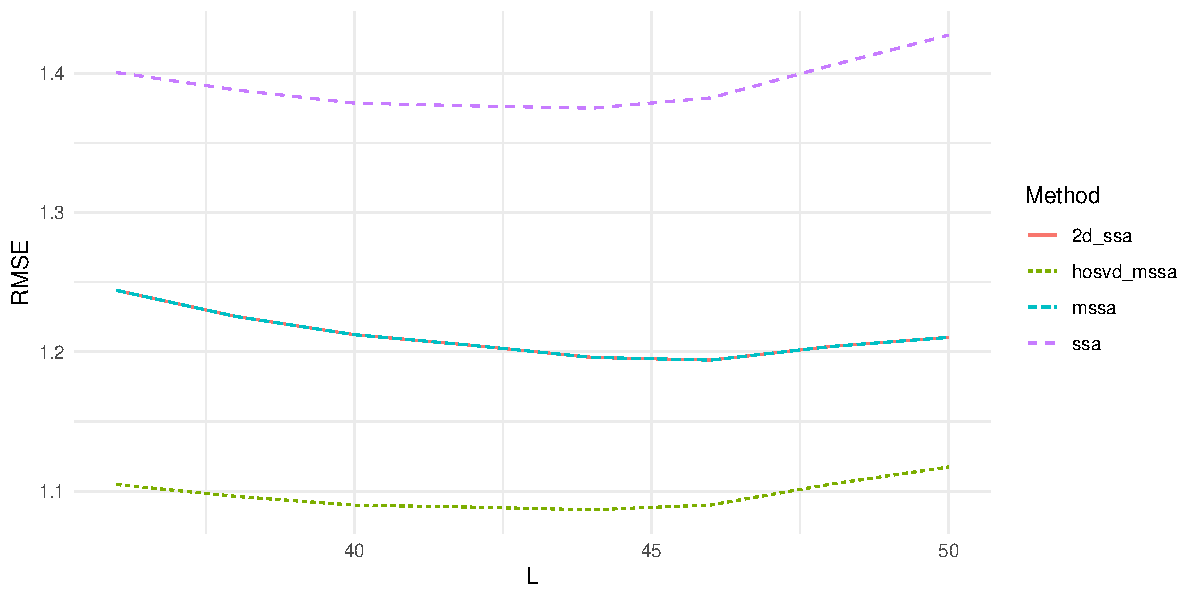
\includegraphics[width=.66\linewidth]{two-series-first}\hfill
            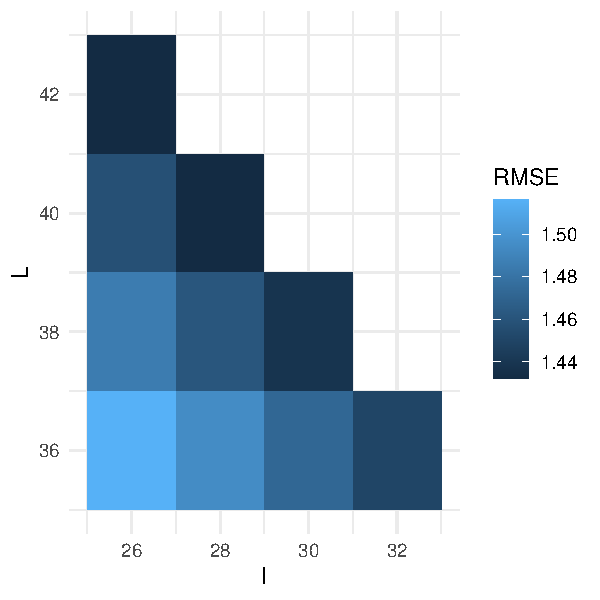
\includegraphics[width=.34\linewidth]{two-series-first_hooi}
            \caption{$\omega_1=\omega_2=1/12$, $\psi_1=\psi_2=0$}
        \end{subfigure} \par\medskip
        \begin{subfigure}{\linewidth}
            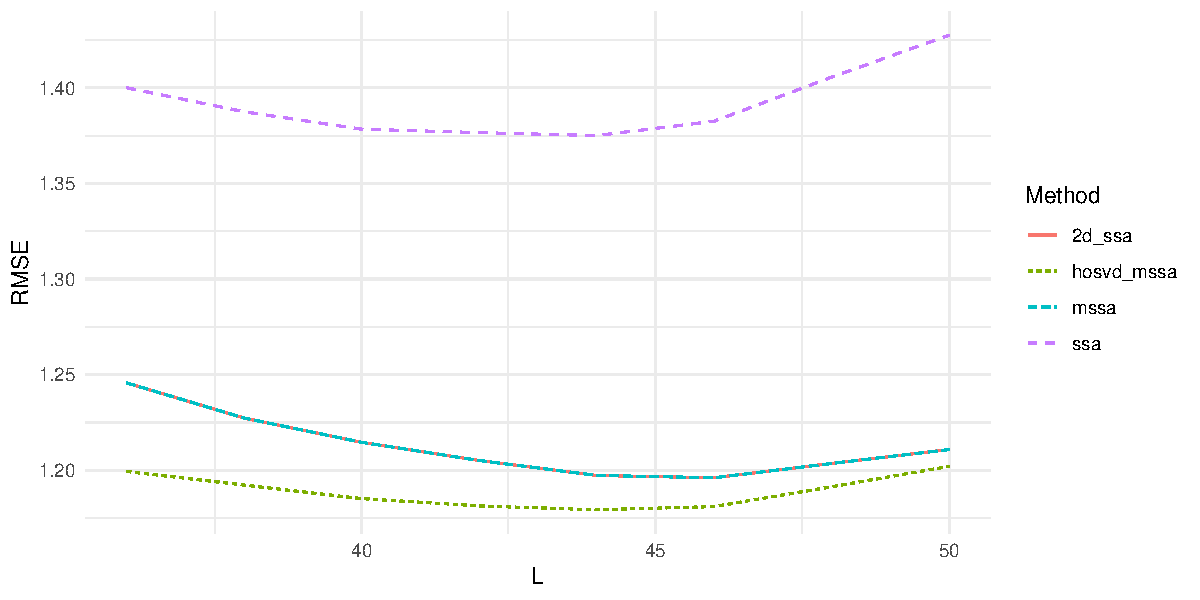
\includegraphics[width=.66\linewidth]{two-series-second}\hfill
            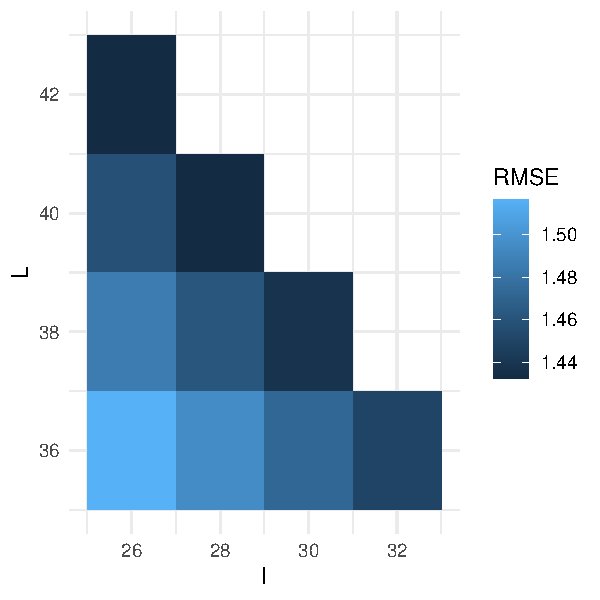
\includegraphics[width=.34\linewidth]{two-series-second_hooi}
            \caption{$\omega_1=\omega_2=1/12$, $\psi_1=0$, $\psi_2=\pi / 4$}
        \end{subfigure}
        \begin{subfigure}{\linewidth}
            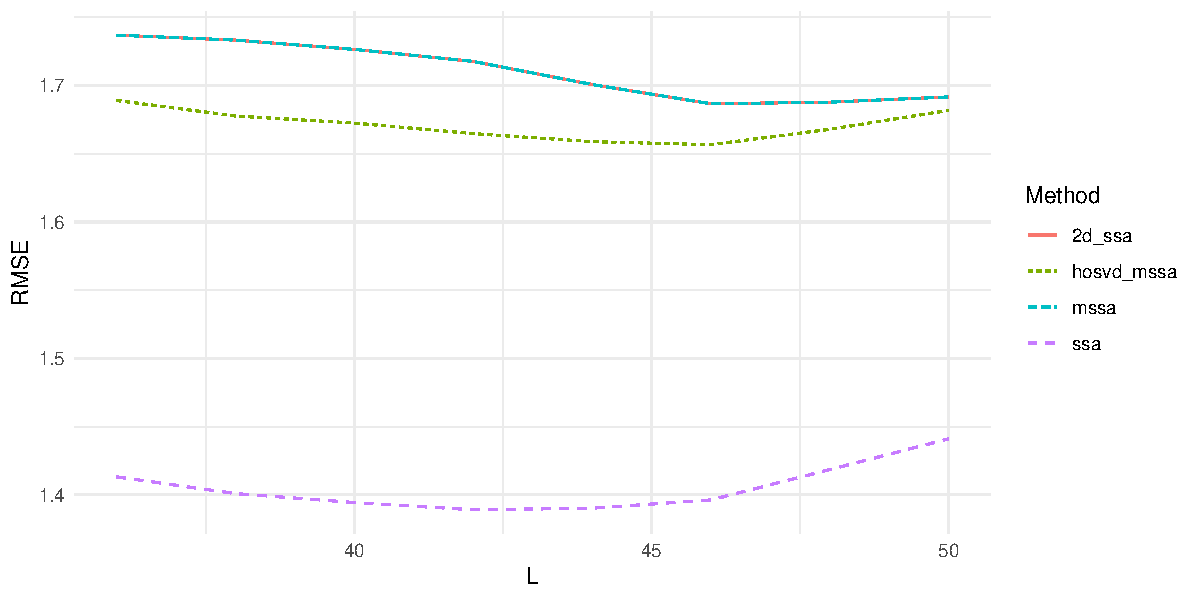
\includegraphics[width=.66\linewidth]{two-series-third}\hfill
            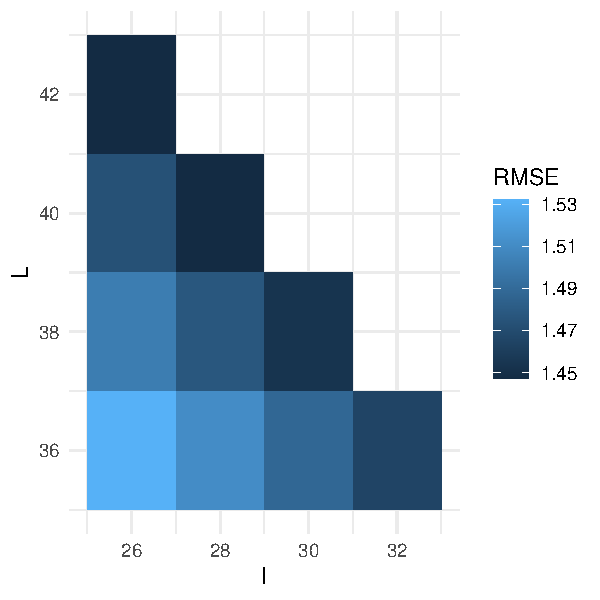
\includegraphics[width=.34\linewidth]{two-series-third_hooi}
            \caption{$\omega_1=1/12$, $\omega_2=1/8$, $\psi_1=0$, $\psi_2=\pi / 4$}
        \end{subfigure}
        \caption{Зависимости точности выделения сигнала от длин окна для каждого из методов
        SSA, MSSA, HOSVD MSSA, 2D-SSA (слева), HOOI SSA (справа), $P=2$, $a_1=30$, $a_2 = 20$.}
        \label{fig:two-series-example}
    \end{figure}
%    \end{example}

%    \begin{example}
%        \label{example:five-series}
%        $P = 5$.

%        В таблице~\ref{tab:ex-five-series-ranks} приведены значения рангов сигналов в каждом из методов
%        в зависимости от значения параметров $a_p$, $\omega_p$, $\psi_p$.
%        Для одномерных методов (SSA и HOOI SSA) указаны ранги каждого одномерного сигнала $\tS^{(p)}$.
%        В таблице~\ref{tab:comparison-five-series} приведены минимальные значения среднеквадратичного отклонения
%        восстановленного сигнала от истинного для каждого метода и при различных значениях параметров.
%        На графиках~\ref{fig:five-series-example} приведены зависимости точности восстановления
%        сигнала от выбора параметра $L$ для методов SSA, MSSA, HOSVD MSSA и 2D-SSA, и от
%        выбора параметров $I, L$ для метода HOOI SSA.
    \begin{table}[!ht]
        \centering
        \caption{Сравнение SSA, HOOI SSA, MSSA, HOSVD MSSA и 2D-SSA: ранги сигнала
        вида~\eqref{eq:general-signal-example}, $P=5$.}
        \begin{tabular}{c|cccc}
            Параметры     & (HOOI) SSA & (HOSVD) MSSA & $r_3$ & 2D-SSA \\
            \hline
            \begin{tabular}{c}
                $a_p=30$     \\
                $\omega_p = \frac 1 {12}$,
                $\psi_p = 0$ \\
            \end{tabular} & 2          & 2            & 1     & 2      \\
            \hline
            \begin{tabular}{c}
                $a_1 = a_4 = 30$ \\
                $a_2 = a_5 =20$,
                $a_3=25$         \\
                $\omega_p = \frac 1 {12}$,
                $\psi_p = 0$     \\
            \end{tabular} & 2          & 2            & 1     & 6      \\
            \hline
            \begin{tabular}{c}
                $a_p=30$,
                $\omega_p = \frac 1 {12}$, \\
                $\psi_p = 2(p-1)\pi / 3$
            \end{tabular} & 2          & 2            & 2     & 2      \\
            \hline
            \begin{tabular}{c}
                $a_p=30$,
                $\psi_p = 2(p-1)\pi / 3$                        \\
                $\omega_1 = \omega_2 = \omega_3 = \frac 1 {12}$ \\
                $\omega_4=\omega_5=\frac 1 8$
            \end{tabular} & 2          & 4            & 4     & 10     \\
            \hline
        \end{tabular}\label{tab:ex-five-series-ranks}
    \end{table}
    \begin{table}[!ht]
        \centering
        \caption{Сравнение SSA, HOOI SSA, MSSA, HOSVD MSSA и 2D-SSA: минимальные RMSE
        оценки сигнала вида~\eqref{eq:general-signal-example}, $P=5$.}
        \begin{tabular}{c|ccccc}
            \hline
            Параметры     & SSA           & HOOI SSA & MSSA & HOSVD MSSA    & 2D-SSA        \\
            \hline
            \begin{tabular}{c}
                $a_p = 30$   \\
                $\omega_p = \frac 1 {12}$,
                $\psi_p = 0$ \\
            \end{tabular} & 1.34          & 0.00     & 0.95 & 0.75          & \textbf{0.73} \\
            \hline
            \begin{tabular}{c}
                $a_1 = a_4 = 30$ \\
                $a_2 = a_5 =20$,
                $a_3=25$         \\
                $\omega_p = \frac 1 {12}$,
                $\psi_p = 0$     \\
            \end{tabular} & 1.38          & 1.41     & 1.07 & \textbf{0.86} & 1.45          \\  \\
            \hline
            \begin{tabular}{c}
                $a_p=30$,
                $\omega_p = \frac 1 {12}$ \\
                $\psi_p = 2(p-1)\pi / 3$
            \end{tabular} & 1.38 & 1.41 & 1.07 & 1.05 & \textbf{0.84} \\
            \hline
            \begin{tabular}{c}
                $a_p=30$,
                $\psi_p = 2(p-1)\pi / 3$                        \\
                $\omega_1 = \omega_2 = \omega_3 = \frac 1 {12}$ \\
                $\omega_4=\omega_5=\frac 1 8$
            \end{tabular} & \textbf{1.38} & 1.41 & 1.50 & 1.49 & 1.78 \\
            \hline
        \end{tabular}\label{tab:comparison-five-series}
    \end{table}
    \begin{figure}
        \centering
        \begin{subfigure}{.95\linewidth}
            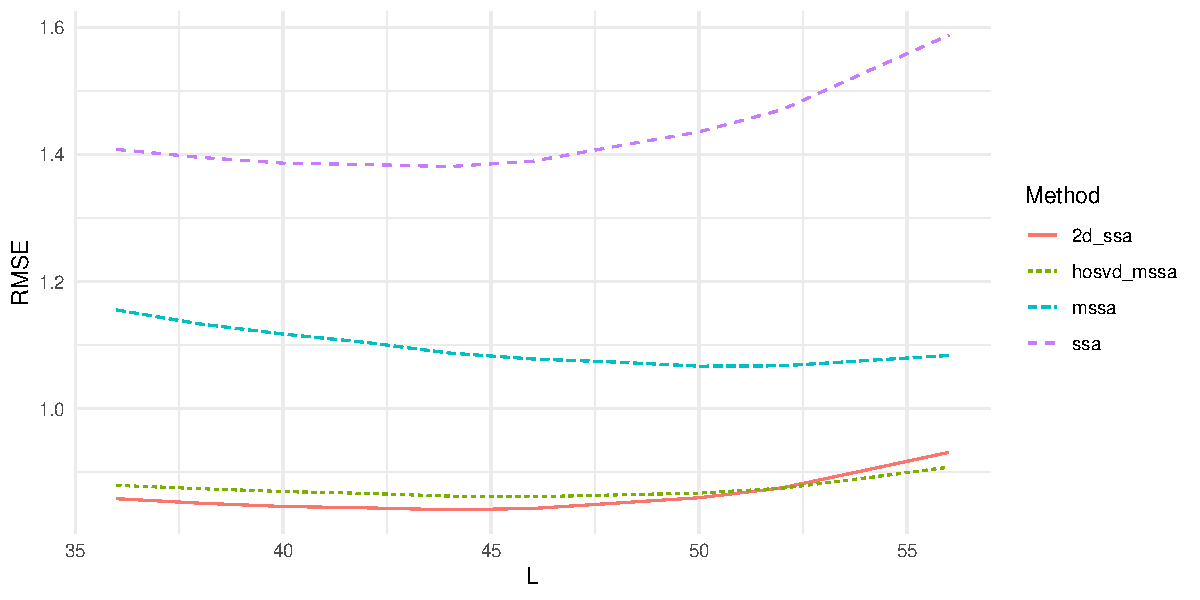
\includegraphics[width=.66\linewidth]{five-series-first}\hfill
            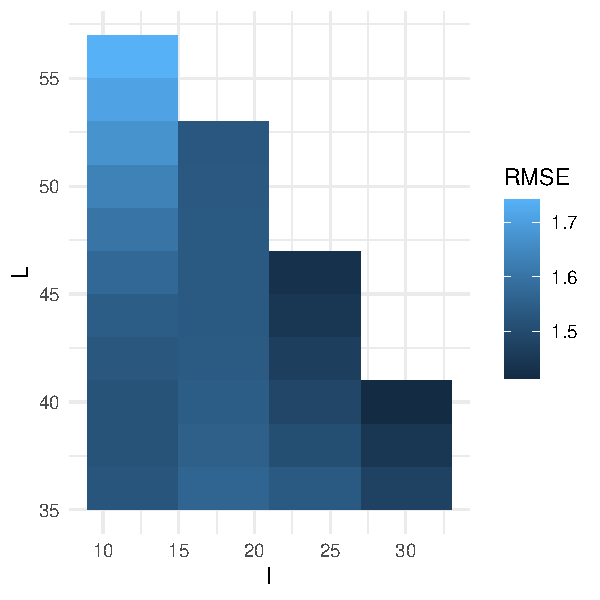
\includegraphics[width=.34\linewidth]{five-series-first_hooi}
            \caption{$a_p = 30$, $\omega_p=1/12$, $\psi_p=0$}
        \end{subfigure} \par\medskip
        \begin{subfigure}{.95\linewidth}
            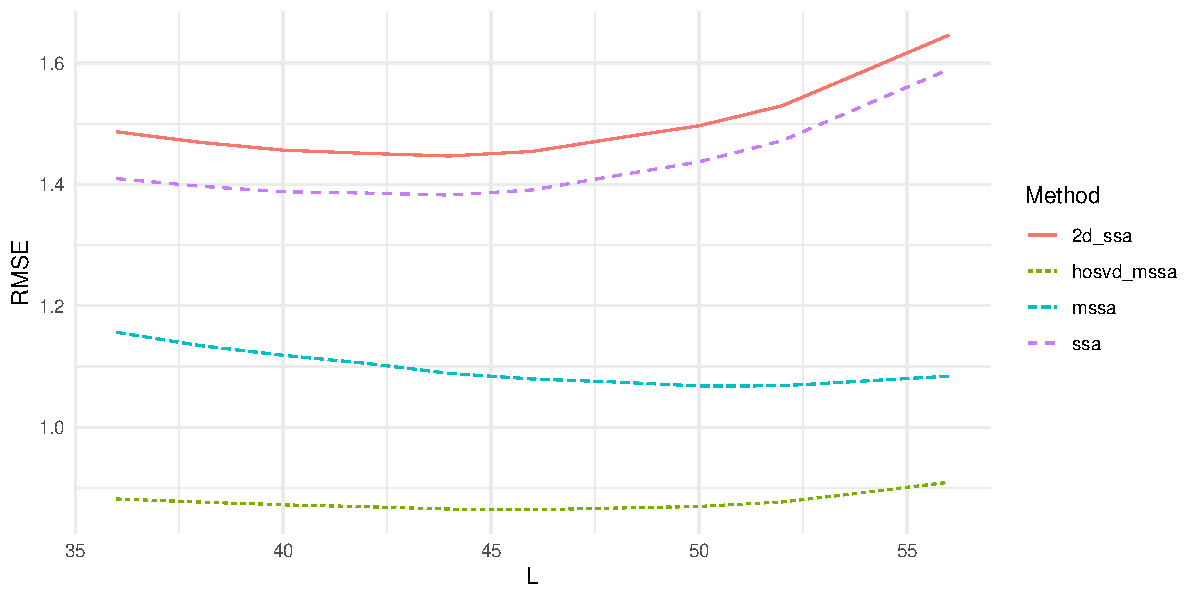
\includegraphics[width=.66\linewidth]{five-series-second}\hfill
            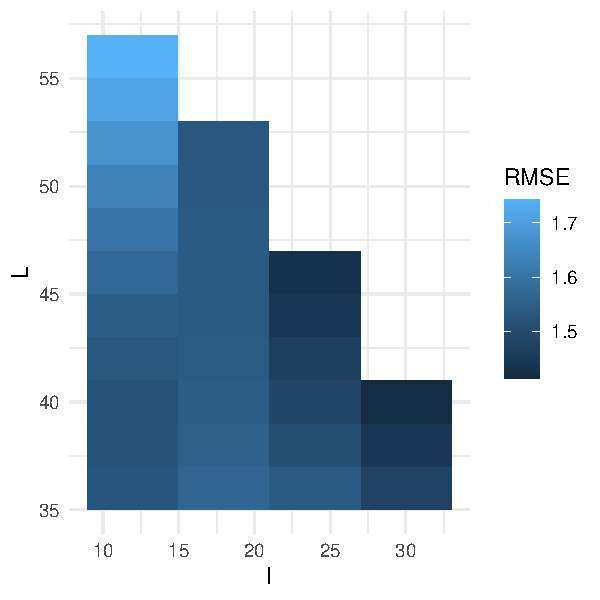
\includegraphics[width=.34\linewidth]{five-series-second_hooi}
            \caption{$a_1=a_4 = 30$, $a_2=a_5=20$, $a_3=25$, $\omega_p=1/12$, $\psi_p=0$}
        \end{subfigure} \par\medskip
        \begin{subfigure}{.95\linewidth}
            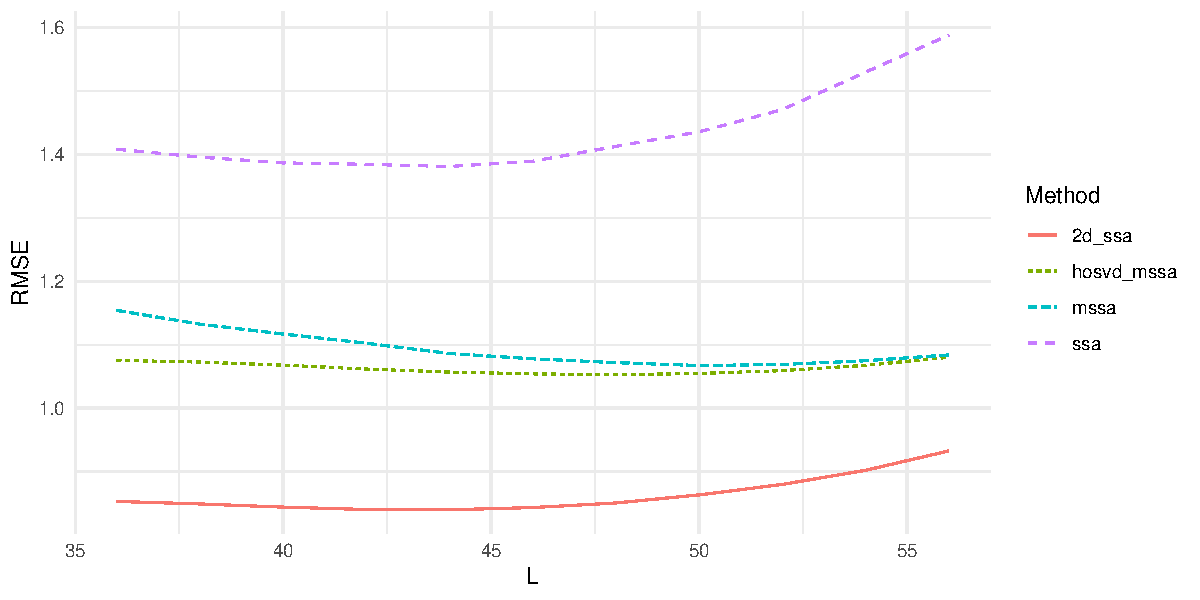
\includegraphics[width=.66\linewidth]{five-series-third}\hfill
            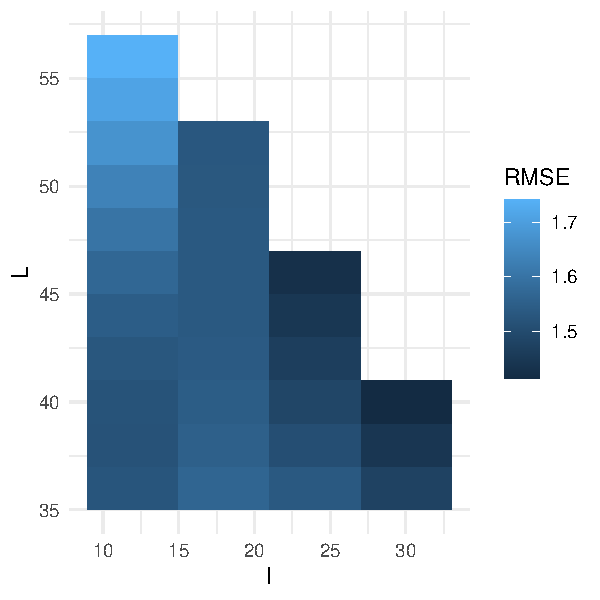
\includegraphics[width=.34\linewidth]{five-series-third_hooi}
            \caption{$a_p = 30$, $\omega_p=1/12$, $\psi_p=2(p-1)\pi/3$}
        \end{subfigure} \par\medskip
        \begin{subfigure}{.95\linewidth}
            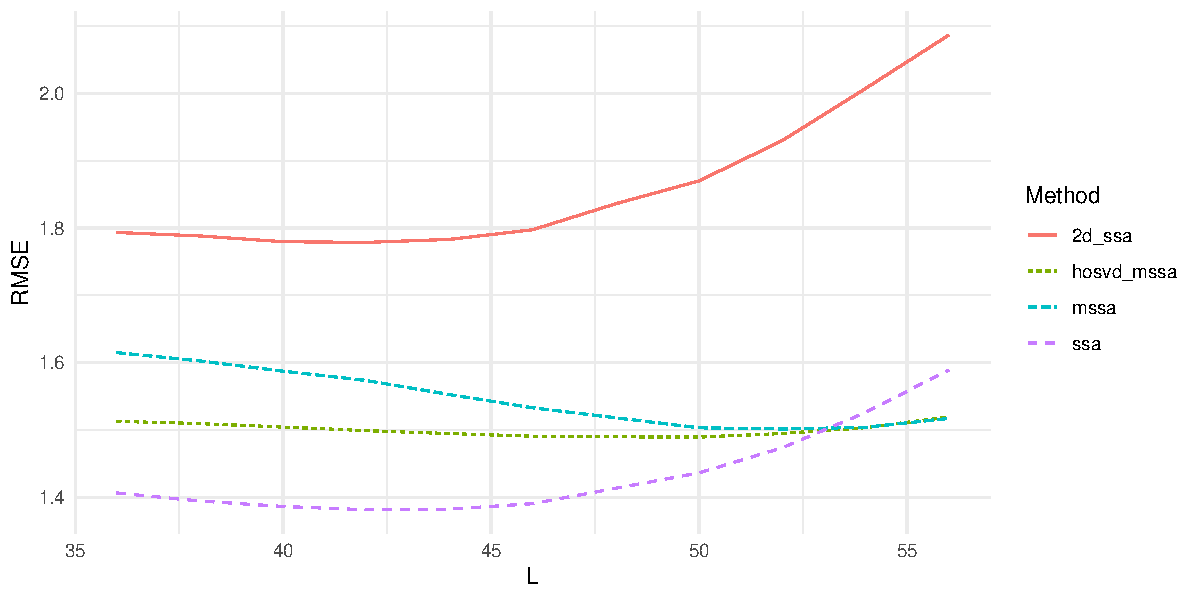
\includegraphics[width=.66\linewidth]{five-series-fourth}\hfill
            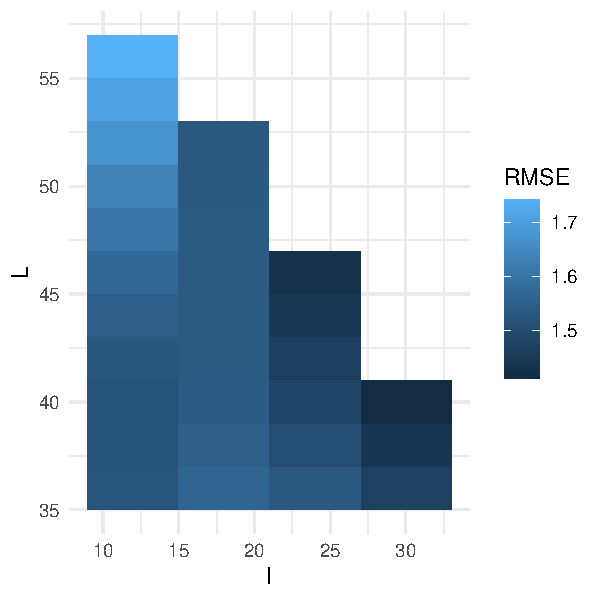
\includegraphics[width=.34\linewidth]{five-series-fourth_hooi}
            \caption{$a_p = 30$, $\omega_1=\omega_2=\omega_3=1/12$, $\omega_4=\omega_5=1/8$, $\psi_p=2(p-1)\pi/3$}
        \end{subfigure}
        \caption{Зависимости точности выделения сигнала от длин окна для каждого из методов
        SSA, MSSA, HOSVD MSSA, 2D-SSA (слева), HOOI SSA (справа), $P=5$.}
        \label{fig:five-series-example}
    \end{figure}
%    \end{example}

%    \begin{example}
%        \label{example:nine-series}
%        $P = 9$.

%        В таблице~\ref{tab:ex-nine-series-ranks} приведены значения рангов сигналов в каждом из методов
%        в зависимости от значения параметров $a_p$, $\omega_p$, $\psi_p$.
%        Для одномерных методов (SSA и HOOI SSA) указаны ранги каждого одномерного сигнала $\tS^{(p)}$.
%        В таблице~\ref{tab:comparison-nine-series} приведены минимальные значения среднеквадратичного отклонения
%        восстановленного сигнала от истинного для каждого метода и при различных значениях параметров.
%        На графиках~\ref{fig:nine-series-example} приведены зависимости точности восстановления
%        сигнала от выбора параметра $L$ для методов SSA, MSSA, HOSVD MSSA и 2D-SSA, и от
%        выбора параметров $I, L$ для метода HOOI SSA.
    \begin{table}[!ht]
        \centering
        \caption{Сравнение SSA, HOOI SSA, MSSA, HOSVD MSSA и 2D-SSA: ранги сигнала
        вида~\eqref{eq:general-signal-example}, $P=9$.}
        \begin{tabular}{c|cccc}
            Параметры     & (HOOI) SSA & (HOSVD) MSSA & $r_3$ & 2D-SSA \\
            \hline
            \begin{tabular}{c}
                $a_p=30$     \\
                $\omega_p = \frac 1 {12}$,
                $\psi_p = 0$ \\
            \end{tabular} & 2          & 2            & 1     & 2      \\
            \hline
            \begin{tabular}{c}
                $a_{p} = a_{p+5} = 30 - 2(p-1)$, $1 \leqslant p \leqslant 4$ \\
                $a_5=22$,
                $\omega_p = \frac 1 {12}$,
                $\psi_p = 0$                                                 \\
            \end{tabular} & 2          & 2            & 1     & 10     \\
            \hline
            \begin{tabular}{c}
                $a_p=30$,
                $\omega_p = \frac 1 {12}$, \\
                $\psi_p = 2(p-1)\pi / 5$
            \end{tabular} & 2          & 2            & 2     & 2      \\
            \hline
            \begin{tabular}{c}
                $a_p=30$,
                $\psi_p = 2(p-1)\pi / 5$                               \\
                $\omega_p = \frac 1 {12}$, $1 \leqslant p \leqslant 7$ \\
                $\omega_8=\omega_9=\frac 1 8$
            \end{tabular} & 2          & 4            & 4     & 10     \\
            \hline
        \end{tabular}\label{tab:ex-nine-series-ranks}
    \end{table}
    \begin{table}[!ht]
        \centering
        \caption{Сравнение SSA, HOOI SSA, MSSA, HOSVD MSSA и 2D-SSA: минимальные RMSE
        оценки сигнала вида~\eqref{eq:general-signal-example}, $P=9$.}
        \begin{tabular}{c|ccccc}
            \hline
            Параметры     & SSA           & HOOI SSA & MSSA & HOSVD MSSA    & 2D-SSA        \\
            \hline
            \begin{tabular}{c}
                $a_p = 30$   \\
                $\omega_p = \frac 1 {12}$,
                $\psi_p = 0$ \\
            \end{tabular} & 1.38          & 1.42     & 1.01 & 0.78          & \textbf{0.65} \\
            \hline
            \begin{tabular}{c}
                $a_{p} = a_{p+5} = 30 - 2(p-1)$ \\
                $1 \leqslant p \leqslant 4$,
                $a_5=22$                        \\
                $\omega_p = \frac 1 {12}$,
                $\psi_p = 0$
            \end{tabular} & 1.38          & 1.42     & 1.01 & \textbf{0.78} & 1.90          \\
            \hline
            \begin{tabular}{c}
                $a_p=30$,
                $\omega_p = \frac 1 {12}$ \\
                $\psi_p = 2(p-1)\pi / 5$
            \end{tabular} & 1.38          & 1.42     & 1.01 & 1.00          & \textbf{0.65} \\
            \hline
            \begin{tabular}{c}
                $a_p=30$,
                $\psi_p = 2(p-1)\pi / 5$                               \\
                $\omega_p = \frac 1 {12}$, $1 \leqslant p \leqslant 7$ \\
                $\omega_8=\omega_9=\frac 1 8$
            \end{tabular} & \textbf{1.39} & 1.42     & 1.42 & 1.42          & 1.42          \\
            \hline
        \end{tabular}\label{tab:comparison-nine-series}
    \end{table}
    \begin{figure}
        \centering
        \begin{subfigure}{.95\linewidth}
            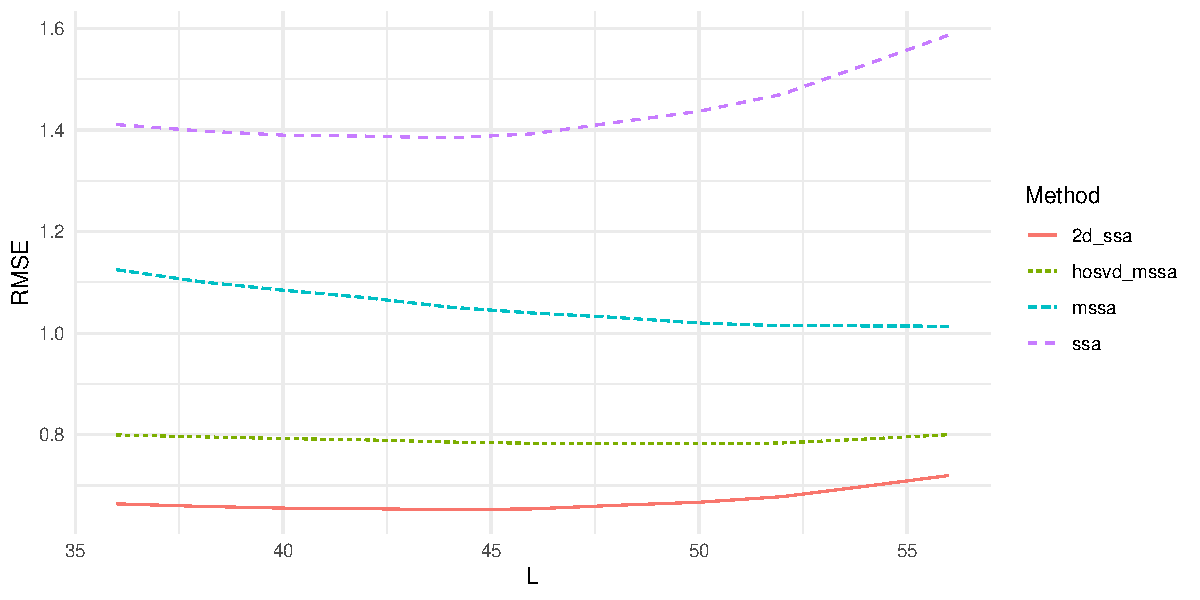
\includegraphics[width=.66\linewidth]{nine-series-first}\hfill
            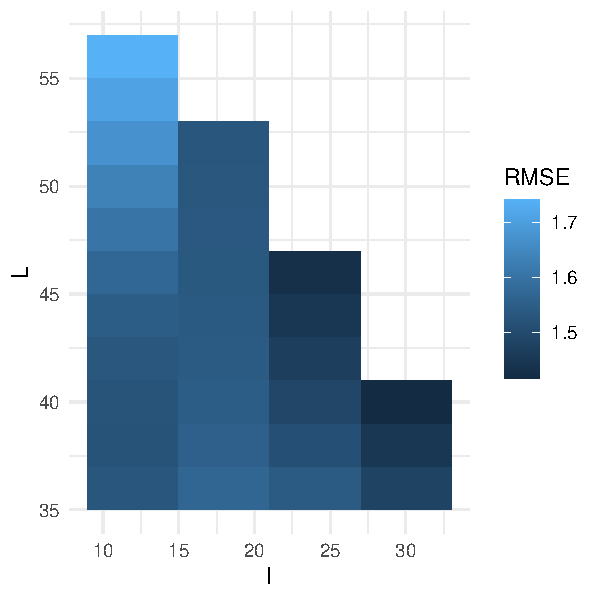
\includegraphics[width=.34\linewidth]{nine-series-first_hooi}
            \caption{$a_p = 30$, $\omega_p=1/12$, $\psi_p=0$}
        \end{subfigure} \par\medskip
        \begin{subfigure}{.95\linewidth}
            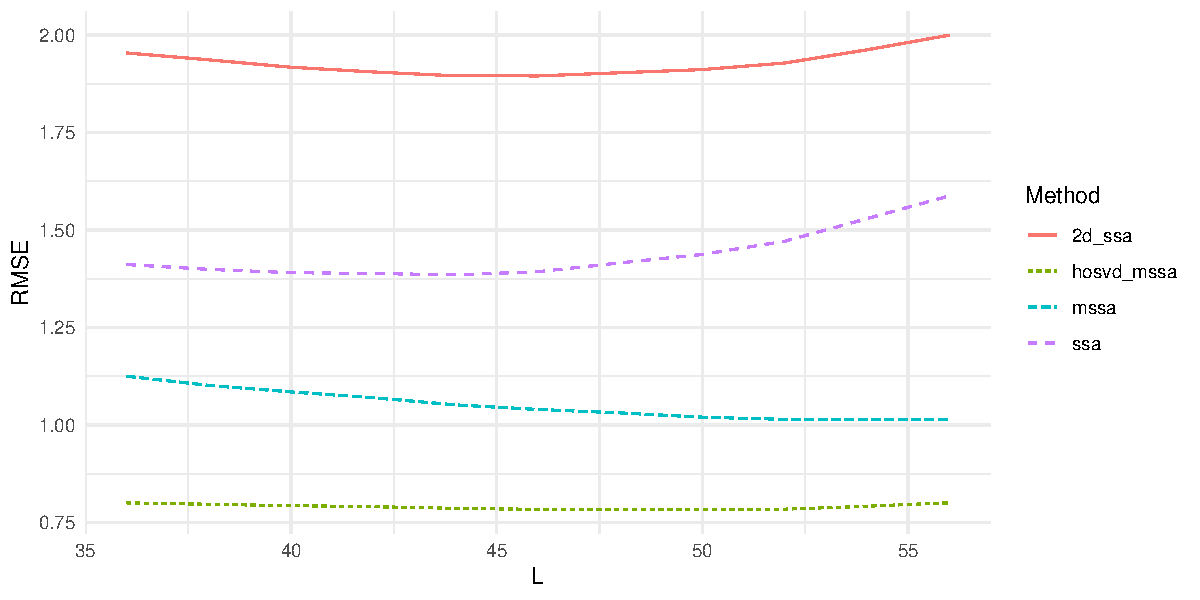
\includegraphics[width=.66\linewidth]{nine-series-second}\hfill
            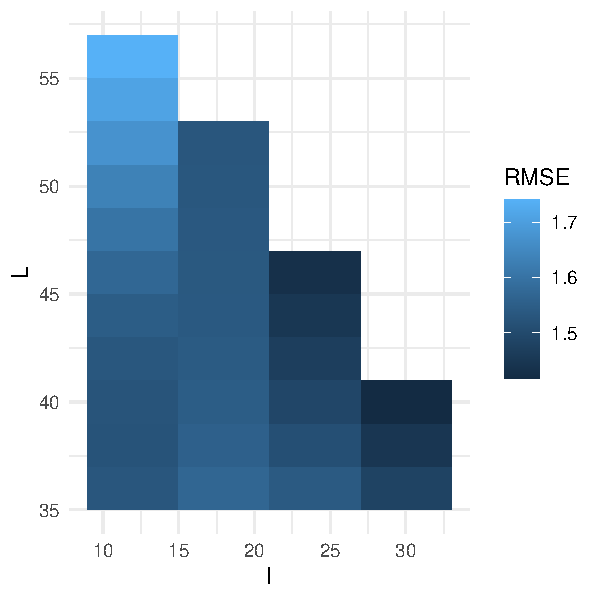
\includegraphics[width=.34\linewidth]{nine-series-second_hooi}
            \caption{$a_{p} = a_{p+5} = 30 - 2(p-1)$, $1 \leqslant p \leqslant 4$,
                $a_5=22$, $\omega_p=1/12$, $\psi_p=0$}
        \end{subfigure} \par\medskip
        \begin{subfigure}{.95\linewidth}
            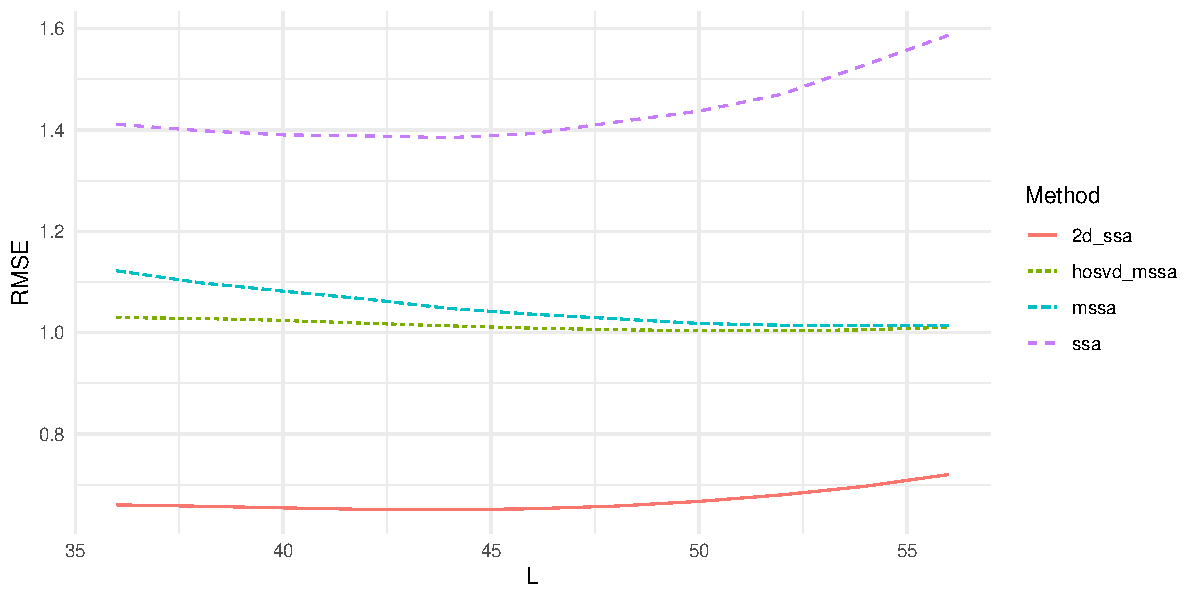
\includegraphics[width=.66\linewidth]{nine-series-third}\hfill
            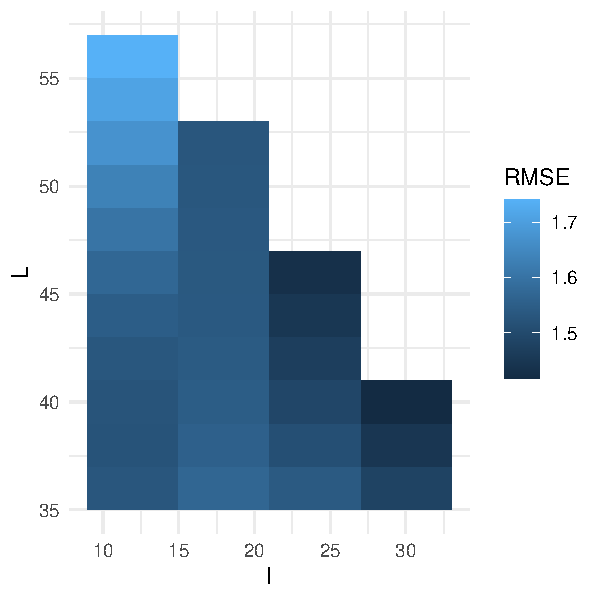
\includegraphics[width=.34\linewidth]{nine-series-third_hooi}
            \caption{$a_p = 30$, $\omega_p=1/12$, $\psi_p=2(p-1)\pi/5$}
        \end{subfigure} \par\medskip
        \begin{subfigure}{.95\linewidth}
            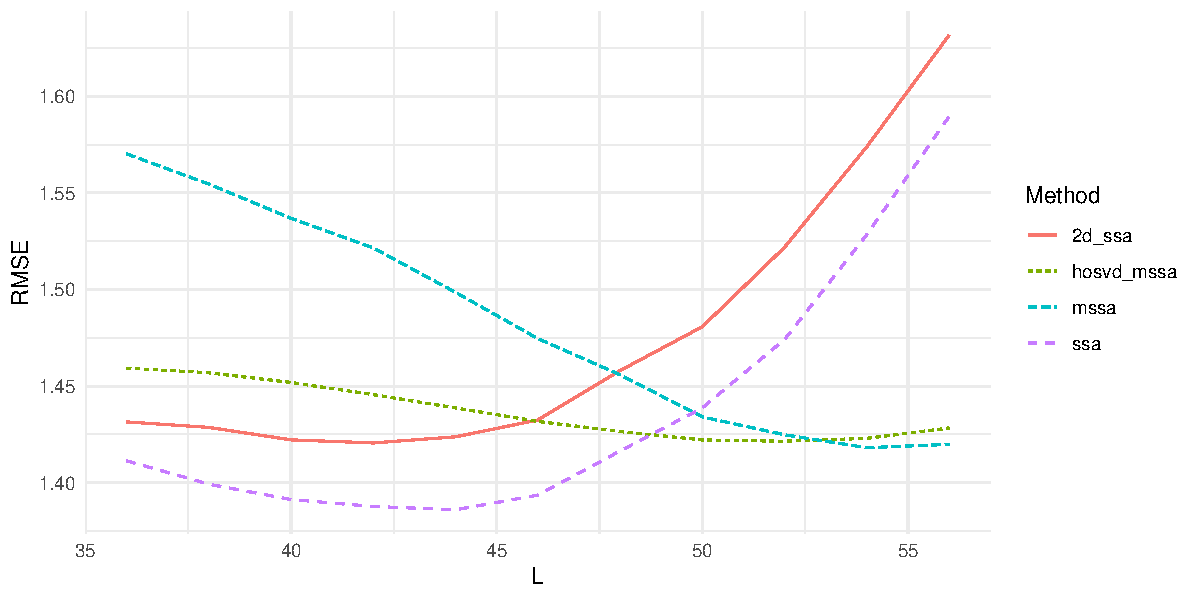
\includegraphics[width=.66\linewidth]{nine-series-fourth}\hfill
            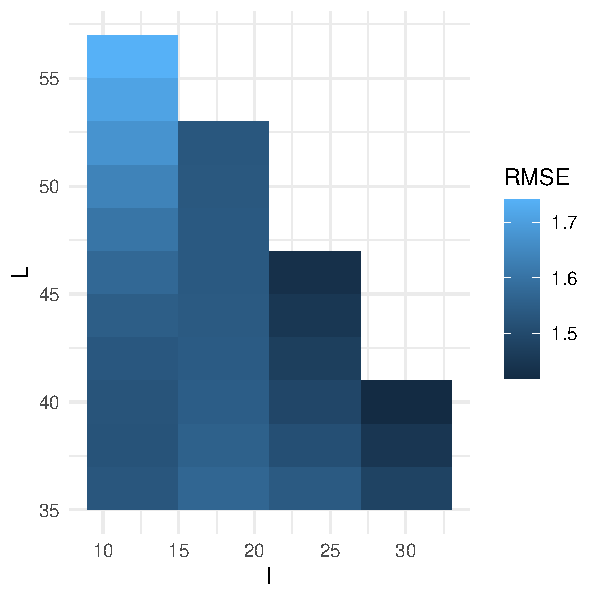
\includegraphics[width=.34\linewidth]{nine-series-fourth_hooi}
            \caption{$a_p = 30$, $\omega_p=1/12$, $1 \leqslant p \leqslant 7$,
                $\omega_8=\omega_9=1/8$, $\psi_p=2(p-1)\pi/5$}
        \end{subfigure}
        \caption{Зависимости точности выделения сигнала от длин окна для каждого из методов
        SSA, MSSA, HOSVD MSSA, 2D-SSA (слева), HOOI SSA (справа), $P=9$.}
        \label{fig:nine-series-example}
    \end{figure}
%\end{example}

    \paragraph{Итоги численного сравнения}\label{par:numerical-comparison-res}
    Таким образом, метод HOSVD MSSA выделил сигнал точнее, чем метод MSSA во всех примерах, и
    оказался точнее метода 2D-SSA в случае малого числа рядов и в случае различающихся
    амплитуд у сигналов, причём последнее преимущество увеличилось с увеличением размерности ряда.
    Однако в случаях равных сигналов и сигналов с меняющейся линейно фазой метод 2D-SSA оказался точнее,
    чем HOSVD MSSA, причём это преимущество увеличилось при увеличении размерности ряда.

    \paragraph{Трудоёмкости алгоритмов}\label{par:alg-complexity}
    Так как шаг разложения является самым трудоёмким шагом в алгоритмах HOSVD SSA и HOSVD MSSA,
    то для оценки трудоёмкости алгоритма достаточно оценить трудоёмкость HOSVD траекторного тензора.
    Оценим трудоёмкость алгоритма HOSVD MSSA, трудоёмкость HOSVD SSA получается аналогично подстановкой
    других обозначений размерностей.

    Из утверждения~\ref{state:hosvd-to-svd} следует, что вычисление HOSVD траекторного тензора размерности ${L\times K \times P}$
    сводится к вычислению SVD на трёх матрицах размерностей $L\times KP,\, K\times LP,\, P\times LK$.
    Вычисление SVD матрицы размерности $m\times n$ имеет асимптотическую трудоёмкость, равную $O(\min(mn^2, m^2 n)).$
    Таким образом, асимптотическая сложность HOSVD траекторного тензора, а следовательно и всего алгоритма, имеет вид
    \begin{equation}
        \label{eq:hosvd-mssa-complexity}
        O\left(LKP(\min(L, KP) + \min(K, LP) + \min(P, LK))\right).
    \end{equation}

    Самым трудоёмким шагом в алгоритме HOOI SSA является применение к траекторному тензору алгоритма HOOI.
    Описание этого алгоритма для приближения тензора размерности $I\times J \times K$
    тензором с $n$-рангами $(r_1, r_2, r_3)$ можно найти в статье~\cite{hooi-algorithm}.
    Этот алгоритм является итерационным, и в обозначениях выше каждая итерация имеет асимптотическую сложность
    \begin{equation}
        \label{eq:hooi-iter-complexity}
        O(r_1^2 \min(I, r_2 r_3) + r_2^2 \min(J, r_1 r_3) + r_3^2 \min(K, r_1 r_2)).
    \end{equation}
    Если предположить, что пользователь задаёт верхнюю границу количества итераций $C$, то асимптотическая
    сложность алгоритма HOOI будет иметь вид~\eqref{eq:hooi-iter-complexity} с константой,
    пропорциональной $C$.


    \section{Альтернативные тензорные разложения}\label{sec:other-decomp}
    Помимо HOSVD, существует ещё один тип тензорных разложений: ранговое разложение тензора.
    Идея заключается в представлении тензора $\mathcal{A}$ в виде линейной комбинации $R$ тензоров ранга $1$, где $R=\operatorname{rank}(\mathcal{A})$.
    Однако нахождение этого ранга в общем случае является NP-трудной задачей~\cite{NP-hard}.

    CANDECOMP-PARAFAC~\cite{parafac1, parafac2}"--- итерационный метод приближения тензора суммой заданного
    пользователем числа тензоров ранга $1$.
    То есть по параметру $K$ этот метод считает наилучшее приближение входного тензора суммой $K$ тензоров ранга $1$.
    Заметим, что из-за отсутствия каких-либо требований к ортогональности в определении рангового разложения тензора,
    многие свойства, верные в теории SSA, могут потерять справедливость при использовании этого разложения.

    Рассмотрим ряды $\tilde{x}_n=3,\, \hat{x}_n=\sin(2\pi n / 3)$, $n \in \overline{0:15}$.
    Построим по этим рядам траекторные тензоры с параметрами $I=L=6$.
    Тогда ранг траекторного тензора $\tilde{\mathcal{X}}$, соответствующего константному ряду, равен $1$, так как его
    можно представить в виде
    \[
        \tilde{\mathcal{X}} = 3 X\circ X \circ X,
    \]
    где $X=(1,\, 1,\, 1,\, 1,\, 1,\, 1)$.
    Ранг траекторного тензора $\hat{\mathcal{X}}$, соответствующего синусу, равен $3$, так как его можно представить в виде
    \[
        \hat{\mathcal{X}}=\sum_{k=1}^{3}\lambda_i X_i \circ Y_i\circ Z_i,
    \]
    где
    \begin{gather*}
        \lambda_1 =160.56,\, \lambda_2 =65.69,\, \lambda_3 =123.76,\\
        \mathbf{X}=[X_1,\, X_2,\, X_3] =
        \begin{pmatrix}
            -0.16 & 0.25  & 0.06  \\
            0.25  & -0.06 & -0.25 \\
            -0.09 & -0.19 & 0.19  \\
            -0.16 & 0.25  & 0.06  \\
            0.25  & -0.06 & -0.25 \\
            -0.09 & -0.19 & 0.19
        \end{pmatrix},\\
        \mathbf{Y}=[Y_1,\, Y_2,\, Y_3] =
        \begin{pmatrix}
            -0.25 & -0.15 & 0.21  \\
            0.18  & -0.10 & -0.25 \\
            0.07  & 0.25  & 0.04  \\
            -0.25 & -0.15 & 0.21  \\
            0.18  & -0.10 & -0.25 \\
            0.07  & 0.25  & 0.04
        \end{pmatrix},\\
        \mathbf{Z}=[Z_1,\, Z_2,\, Z_3] =
        \begin{pmatrix}
            -0.10 & -0.25 & -0.01 \\
            0.25  & 0.12  & -0.24 \\
            -0.15 & 0.13  & 0.25  \\
            -0.10 & -0.25 & -0.01 \\
            0.25  & 0.12  & -0.24 \\
            -0.15 & 0.13  & 0.25
        \end{pmatrix},
    \end{gather*}
    притом точных приближений двумя тензорами ранга $1$ нет.

    Траекторный тензор ряда $x_n=\tilde{x}_n+\hat{x}_n$, построенный с параметрами $I=L=6$ представим в виде суммы
    \[
        \mathcal{X}=\sum_{k=1}^{4}\lambda_i X_i \circ Y_i\circ Z_i,
    \]
    где
    \begin{gather*}
        \lambda_1 =320.17,\, \lambda_2 =120.97,\, \lambda_3 =209.38,\, \lambda_4=648\\
        \mathbf{X}=[X_1,\, X_2,\, X_3,\, X_4] =
        \begin{pmatrix}
            -0.25 & -0.25 & 0.25  & -0.17 \\
            0.11  & 0.25  & -0.04 & -0.17 \\
            0.14  & 0.00  & -0.21 & -0.17 \\
            -0.25 & -0.25 & 0.25  & -0.17 \\
            0.11  & 0.25  & -0.04 & -0.17 \\
            0.14  & 0.00  & -0.21 & -0.17
        \end{pmatrix},\\
        \mathbf{Y}=[Y_1,\, Y_2,\, Y_3,\, Y_4] =
        \begin{pmatrix}
            0.25  & -0.25 & -0.25 & -0.17 \\
            -0.08 & 0.21  & -0.00 & -0.17 \\
            -0.17 & 0.04  & 0.25  & -0.17 \\
            0.25  & -0.25 & -0.25 & -0.17 \\
            -0.08 & 0.21  & -0.00 & -0.17 \\
            -0.17 & 0.04  & 0.25  & -0.17
        \end{pmatrix},\\
        \mathbf{Z}=[Z_1,\, Z_2,\, Z_3,\, Z_4] =
        \begin{pmatrix}
            -0.00 & -0.14 & -0.08 & 0.17 \\
            -0.25 & -0.11 & 0.25  & 0.17 \\
            0.25  & 0.25  & -0.17 & 0.17 \\
            -0.00 & -0.14 & -0.08 & 0.17 \\
            -0.25 & -0.11 & 0.25  & 0.17 \\
            0.25  & 0.25  & -0.17 & 0.17
        \end{pmatrix},
    \end{gather*}
    притом точных приближений тремя тензорами ранга $1$ нет.

    По виду векторов видно, что четвёртая компонента разложения соответствует константному ряду, а остальные три имеют период равный $3$.
    Таким образом, несмотря на отсутствие ограничений на ортогональность в определении ранговых разложений тензора, наблюдается
    отделимость константного ряда от периодического ряда при наличии условий слабой разделимости в терминах SSA и отсутствия
    шума.
    Однако понятия ранга в терминах SSA и в терминах CPD различаются, так как в терминах SSA синус с периодом $3$ имеет ранг $2$, а в
    терминах рангового разложения, как показано выше, такой синус имеет ранг $3$.

    Другим недостатком CPD является то, что это итерационный метод, причём процесс итерации начинается
    с генерации случайной матрицы, в связи с чем на одних и тех же данных он может выдавать разные результаты, в том
    числе может как сойтись, так и нет.

    Возможно можно добиться лучших результатов, используя CPD или его модификации, если строить тензор по ряду другим образом и подбирать
    другие параметры разложения.
    Этот вопрос предлагается изучить в будущих работах.
    \newpage


    \section{Заключение}\label{sec:conclusion}
    В работе было показано, что по своим свойствам HO-SSA и HOSVD MSSA c использованием HOSVD
    имеют много общего с Basic SSA и MSSA соответственно.
    Однако, есть и особенности, кардинально меняющие свойства методов, которые можно использовать для анализа временных рядов.

    В результате исследования методов HO-SSA и HOSVD MSSA c HOSVD были сделаны следующие выводы:
    методы можно использовать для выделения сигнала, однако остался неизученным вопрос о том,
    как с их помощью разделять компоненты сигнала.
    Также, в большинстве случаев, как HOSVD SSA, так и HOOI SSA, оказались хуже,
    чем Basic SSA в точности выделения сигнала.
    Удалось построить только один пример, где Basic SSA менее точно выделяет сигнал.
    Это противоречит результатам работы~\cite{hosvd-hooi-separation}, где показано преимущество Tensor SSA с
    использованием HOOI.
    Однако, в этой статье сравнение идет для сигнала в виде суммы двух комплексных экспонент по точности оценке частоты сигналов.

    С другой стороны, метод HOSVD MSSA выделил сигнал точнее метода MSSA во всех рассмотренных случаях, но в
    некоторых из них данный метод оказался менее точным, чем метод 2D-SSA.

    Таким образом, остались открытыми вопросы: подтвердить преимущество HOSVD-SSA для оценивания
    частот сигнала,
    о котором утверждается в статье~\cite{hosvd-hooi-separation}, найти методы, которые разделяют компоненты сигнала,
    например в работе~\cite{cpd-separation} предлагается метод CPD для разделения комплексных экспонент, а также
    расширить теорию HOSVD MSSA.

    \bibliography{main}
    \bibliographystyle{ugost2008}

\end{document}
